\chapter{CÀI ĐẶT, TRUY VẤN VÀ KIỂM THỬ}

\section{Tổ chức script và cách chạy}

Toàn bộ cơ sở dữ liệu được tạo bằng các script T-SQL trong thư mục \texttt{db/}
(Bảng~\ref{tab:scripts}). Tệp \texttt{full\_setup.sql} là bản ghép của các tệp 00--09, nên
chỉ cần mở một tệp trong SSMS và chạy là có CSDL hoàn chỉnh cùng dữ liệu mẫu. Trên máy phát
triển (SQL Server 2025 Express), việc này mất khoảng 4,9 giây.

\begin{table}[H]
\centering
\caption{Các script trong thư mục \texttt{db/}}
\label{tab:scripts}
\renewcommand{\arraystretch}{1.15}
\begin{tabularx}{\textwidth}{>{\raggedright\arraybackslash}p{5.0cm} >{\raggedright\arraybackslash}X}
\toprule
\textbf{Tệp} & \textbf{Nội dung} \\
\midrule
\texttt{00\_database.sql} & Tạo lại CSDL \texttt{video\_archive}, collation \texttt{Latin1\_General\_100\_CI\_AS}, mức tương thích 140 (SQL Server 2017) \\
\texttt{01\_fold\_function.sql} & Hàm bỏ dấu \texttt{fn\_fold\_vi} (cần có trước các bảng) \\
\texttt{02\_tables.sql} & 30 bảng, 1 \texttt{SEQUENCE}, ràng buộc đặt tên và chỉ mục \\
\texttt{03\_functions.sql} & \texttt{fn\_tokens}, \texttt{fn\_nearest\_keyframe}, \texttt{fn\_has\_permission}, \texttt{fn\_topic\_subtree} \\
\texttt{04\_views.sql} & 11 view \\
\texttt{05\_procedures.sql} & 10 thủ tục lưu trữ \\
\texttt{06\_triggers.sql} & 6 trigger ghi nhật ký \\
\texttt{07\_seed.sql} & Quyền, vai trò, cây chủ đề, nguồn tìm kiếm, từ dừng \\
\texttt{08\_security.sql} & Role và người dùng CSDL, cấp quyền \\
\texttt{09\_sample\_data.sql} & Dữ liệu mẫu L23 (sinh tự động), cuối tệp gọi \texttt{sp\_rebuild\_text\_index} \\
\texttt{10\_queries.sql} & 25 truy vấn nghiệp vụ (chỉ đọc) \\
\texttt{11\_tests.sql} & Kiểm thử ràng buộc, giao dịch, phân quyền, chỉ mục, nhất quán (luôn rollback) \\
\texttt{full\_setup.sql} & Ghép 00--09 thành một tệp \\
\texttt{migrations/001\_...} & Thêm \texttt{sp\_register\_reader} vào CSDL đã tạo từ bản trước (có bản \texttt{\_down} để gỡ) \\
\bottomrule
\end{tabularx}
\end{table}

Một số lưu ý khi viết script cho SQL Server:
\begin{itemize}
    \item Mọi tệp lưu dạng UTF-8 có BOM để SSMS đọc đúng tiếng Việt, và mọi chuỗi tiếng Việt
    có tiền tố \texttt{N'...'}; thiếu tiền tố thì chuỗi bị đổi sang bảng mã một byte và mất dấu.
    \item Mỗi câu \texttt{CREATE FUNCTION/PROCEDURE/VIEW/TRIGGER} phải đứng đầu một lô lệnh,
    nên các đối tượng được ngăn bằng \texttt{GO}.
    \item Cột tính toán \texttt{PERSISTED} và chỉ mục trên nó đòi hỏi
    \texttt{SET QUOTED\_IDENTIFIER ON} và \texttt{SET ANSI\_NULLS ON}; sqlcmd mặc định tắt
    tuỳ chọn đầu nên phải chạy với \texttt{-I} hoặc đặt ở đầu script.
    \item Một lệnh \texttt{INSERT ... VALUES} chỉ được tối đa 1.000 dòng, nên bộ sinh dữ liệu
    mẫu chia 5.913 khung hình thành 6 lệnh.
\end{itemize}

Trong báo cáo, các đoạn mã được rút gọn và bỏ chú thích. Một số chuỗi thông báo tiếng Việt
trong mã được viết lại bằng tiếng Anh vì gói \texttt{listings} của \LaTeX{} không hiển thị
được ký tự tiếng Việt. Mã nguồn đầy đủ nằm trong thư mục \texttt{db/}.

Dữ liệu mẫu được sinh bằng lệnh \texttt{footage sample --batches L23}. Bộ sinh đọc
\texttt{frames.csv}, các tệp OCR, ASR và tệp yêu cầu mẫu \texttt{labels/l23\_requests.csv},
nhân đôi dấu nháy, gộp khoảng trắng rồi ghi ra các câu \texttt{INSERT}. Phần danh mục minh
hoạ (Chương 1) được sinh theo quy tắc cố định để chạy lại cho cùng kết quả:
\begin{itemize}
    \item 5 đơn vị, 5 bộ sưu tập, 5 tài khoản demo (mật khẩu băm sẵn). Khoá ngoại được nối
    bằng mã (\texttt{org\_code}, \texttt{username}) qua \texttt{INSERT ... SELECT ... JOIN},
    không phụ thuộc giá trị \texttt{IDENTITY}.
    \item Yêu cầu thứ $i$ do ba bạn đọc gửi lần lượt, gửi cách thời điểm nạp $125 - i$ ngày.
    Một nửa số yêu cầu có một đoạn tư liệu do \texttt{thuthu1} chọn tại vị trí đã xác minh;
    một nửa trong số đó được cấp phép sau 2--8 ngày, thời hạn 30, 90, 180 hoặc 365 ngày; 6 yêu
    cầu chưa có đoạn nào bị từ chối; còn lại chờ xử lý.
    \item Chủ đề được gắn bằng một câu \texttt{INSERT ... SELECT DISTINCT} nối bảng luật
    (chủ đề, mẫu \texttt{LIKE}) với \texttt{asr\_segments.text\_folded}, nên mọi nhãn đều
    xuất phát từ lời nói thật.
\end{itemize}

\section{Hàm người dùng định nghĩa}

\subsection{Hàm bỏ dấu \texttt{fn\_fold\_vi}}

Chữ OCR thường mất dấu (``GIAY'' thay vì ``GIÂY''), còn người dùng gõ có dấu. Để hai bên
khớp nhau, cả văn bản lẫn mô tả cần tìm đều được viết thường và bỏ dấu. Hàm dùng
\texttt{TRANSLATE} để ánh xạ từng ký tự trong 67 nguyên âm có dấu và chữ ``đ'' sang ký tự
không dấu ở cùng vị trí:

\begin{Verbatim}[fontsize=\scriptsize, frame=single]
CREATE OR ALTER FUNCTION dbo.fn_fold_vi (@text NVARCHAR(4000))
RETURNS NVARCHAR(4000)
WITH SCHEMABINDING
AS
BEGIN
    RETURN TRANSLATE(LOWER(@text),
        N'àáạảãâầấậẩẫăằắặẳẵèéẹẻẽêềếệểễìíịỉĩòóọỏõôồốộổỗơờớợởỡùúụủũưừứựửữỳýỵỷỹđ',
        N'aaaaaaaaaaaaaaaaaeeeeeeeeeeeiiiiiooooooooooooooooouuuuuuuuuuuyyyyyd');
END;
\end{Verbatim}

\texttt{WITH SCHEMABINDING} cùng việc chỉ dùng các hàm tất định (\texttt{LOWER},
\texttt{TRANSLATE}) khiến SQL Server đánh dấu hàm là tất định
(\texttt{OBJECTPROPERTY(..., 'IsDeterministic') = 1}). Nhờ vậy hàm được dùng trong cột tính
toán \texttt{PERSISTED} \texttt{text\_folded}. Ví dụ, \texttt{fn\_fold\_vi(N'ĐƯỜNG Hồ Chí
Minh')} trả về \texttt{duong ho chi minh}.

\subsection{Hàm bảng \texttt{fn\_tokens}}

Hàm bảng nội tuyến (inline TVF) tách một đoạn văn thành tập từ khoá: bỏ dấu, đổi dấu câu
thành khoảng trắng bằng \texttt{TRANSLATE}, tách bằng \texttt{STRING\_SPLIT}, bỏ từ một ký
tự và các từ dừng trong bảng \texttt{stopwords}. Cột kết quả dùng collation nhị phân
\texttt{Latin1\_General\_100\_BIN2} để so khớp chính xác với \texttt{terms.term}.
Văn bản (khi lập chỉ mục) và mô tả cần tìm (khi tìm) đều đi qua cùng một hàm, nên hai phía
luôn tách từ giống hệt nhau. Ví dụ, câu ``Trong đoạn tường thuật cuộc đua xe đạp, linh vật
mặc áo vàng giơ bảng số 2!'' cho 14 từ khoá: \texttt{ao, bang, cuoc, dap, dua, gio, linh,
mac, so, thuat, tuong, vang, vat, xe}. Các từ ``trong'', ``đoạn'' là từ dừng; ``2'' chỉ có
một ký tự.

\subsection{Hàm \texttt{fn\_nearest\_keyframe} và \texttt{fn\_has\_permission}}

\texttt{fn\_nearest\_keyframe} trả về khung hình gần một thời điểm nhất trong một video.
Thay vì sắp xếp cả video theo khoảng cách, hàm dò chỉ mục
\texttt{UQ\_keyframes\_video\_time} hai lần, một lần lùi và một lần tiến:

\begin{lstlisting}[caption={Hàm fn\_nearest\_keyframe}, label={lst:nearest}]
CREATE OR ALTER FUNCTION dbo.fn_nearest_keyframe (@video_id VARCHAR(16), @time DECIMAL(10,3))
RETURNS INT
AS
BEGIN
    DECLARE @before_id INT, @before_t DECIMAL(10,3), @after_id INT, @after_t DECIMAL(10,3);
    SELECT TOP (1) @before_id = keyframe_id, @before_t = pts_time
    FROM dbo.keyframes WHERE video_id = @video_id AND pts_time <= @time
    ORDER BY pts_time DESC;
    SELECT TOP (1) @after_id = keyframe_id, @after_t = pts_time
    FROM dbo.keyframes WHERE video_id = @video_id AND pts_time >= @time
    ORDER BY pts_time ASC;
    IF @before_id IS NULL RETURN @after_id;
    IF @after_id IS NULL RETURN @before_id;
    RETURN CASE WHEN @time - @before_t <= @after_t - @time
                THEN @before_id ELSE @after_id END;
END;
\end{lstlisting}

Hàm này gắn mỗi đoạn lời nói vào khung hình gần điểm giữa của đoạn, cả trong thủ tục tìm
kiếm lẫn truy vấn Q14. \texttt{fn\_has\_permission(@user\_id, @permission)} trả về 1 nếu
người dùng đang hoạt động và có quyền qua ít nhất một vai trò; các thủ tục ghi dữ liệu
dùng hàm này để tự kiểm tra quyền.

\subsection{Hàm bảng đệ quy \texttt{fn\_topic\_subtree}}

Cây chủ đề được lưu bằng khoá ngoại tự tham chiếu \texttt{parent\_topic\_id}. Để lấy một
chủ đề cùng mọi chủ đề con cháu ở mọi độ sâu, hàm bảng nội tuyến dùng CTE đệ quy: phần neo
chọn chủ đề gốc, phần đệ quy nối các chủ đề có cha nằm trong tập đã tìm được, cho đến khi
không còn dòng mới. Cột \texttt{path} ghép đường dẫn từ gốc để sắp xếp khi in cây.

\begin{lstlisting}[caption={Hàm fn\_topic\_subtree với CTE đệ quy}, label={lst:subtree}]
CREATE OR ALTER FUNCTION dbo.fn_topic_subtree (@root_id SMALLINT)
RETURNS TABLE
AS
RETURN
    WITH tree AS (
        SELECT t.topic_id, t.topic_name, t.parent_topic_id, 0 AS depth,
               CAST(t.topic_name AS NVARCHAR(1000)) AS path
        FROM dbo.topics t
        WHERE t.topic_id = @root_id
        UNION ALL
        SELECT c.topic_id, c.topic_name, c.parent_topic_id, p.depth + 1,
               CAST(CONCAT(p.path, N' > ', c.topic_name) AS NVARCHAR(1000))
        FROM dbo.topics c
        JOIN tree p ON c.parent_topic_id = p.topic_id
    )
    SELECT topic_id, topic_name, parent_topic_id, depth, path FROM tree;
\end{lstlisting}

Gọi với chủ đề ``Đua xe đạp'' trả về 13 dòng ở ba mức (0--2). Truy vấn Q19 dùng hàm hai lần
để đếm số video của mỗi nhánh, tính cả các chủ đề con.

\section{Thủ tục lưu trữ}

Bảng~\ref{tab:procedures} liệt kê mười thủ tục. Người đang thao tác được ứng dụng đặt vào
ngữ cảnh phiên bằng \texttt{sp\_set\_session\_context N'app\_user\_id', <id>, @read\_only = 1}.
Vì vậy các thủ tục ghi không nhận \texttt{user\_id} qua tham số, tức không tin vào giá trị do
bên gọi tự khai.

\begin{table}[H]
\centering
\caption{Các thủ tục lưu trữ}
\label{tab:procedures}
\renewcommand{\arraystretch}{1.15}
\begin{tabularx}{\textwidth}{>{\raggedright\arraybackslash}p{4.3cm} >{\raggedright\arraybackslash}X}
\toprule
\textbf{Thủ tục} & \textbf{Nghiệp vụ} \\
\midrule
\texttt{sp\_search\_footage} & Tìm khung hình: tách từ mô tả cần tìm, tra chỉ mục ngược OCR/ASR có trọng số IDF, nhận danh sách hình ảnh dạng JSON, gộp bằng RRF \\
\texttt{sp\_submit\_request} & Bạn đọc gửi yêu cầu khai thác; mã yêu cầu lấy từ \texttt{SEQUENCE}; kiểm tra quyền \texttt{request.submit} \\
\texttt{sp\_add\_selection} & Chọn đoạn tư liệu cho yêu cầu (hoặc cập nhật ghi chú); kiểm tra quyền \texttt{selection.write} và trạng thái yêu cầu \\
\texttt{sp\_remove\_selection} & Bỏ đoạn đã chọn; kiểm tra quyền và trạng thái \\
\texttt{sp\_grant\_license} & Duyệt yêu cầu: tạo giấy phép và đổi trạng thái trong một giao dịch \\
\texttt{sp\_reject\_request} & Từ chối yêu cầu đang chờ \\
\texttt{sp\_create\_user} & Tạo tài khoản (kèm đơn vị, đối tượng) và gán vai trò trong một giao dịch \\
\texttt{sp\_register\_reader} & Khách tự đăng ký: luôn chỉ cấp vai trò \texttt{reader} (mục~\ref{sec:register}) \\
\texttt{sp\_progress\_report} & Báo cáo tiến độ, trả kết quả qua ba tham số \texttt{OUTPUT} \\
\texttt{sp\_rebuild\_text\_index} & Lập lại chỉ mục ngược từ toàn bộ OCR và ASR \\
\bottomrule
\end{tabularx}
\end{table}

\subsection{Thủ tục tìm kiếm \texttt{sp\_search\_footage}}

Thủ tục nhận mô tả cần tìm \texttt{@query}, danh sách hình ảnh \texttt{@visual} (mảng JSON
\texttt{keyframe\_id} đã xếp hạng, do ứng dụng lấy từ SigLIP2 và FAISS), các cờ bật/tắt
nguồn, kích thước tập ứng viên \texttt{@pool} và số kết quả \texttt{@top\_k}. Các bước:

\begin{enumerate}
    \item Tách từ khoá của mô tả bằng \texttt{fn\_tokens} và tra mã trong
    \texttt{terms}.
    \item Với mỗi nguồn văn bản, tính điểm của mỗi khung hình (hoặc đoạn lời nói) là tổng
    IDF~\cite{manning2008ir} của các từ khoá khớp, với $N$ là số tài liệu của nguồn và
    $\mathrm{df}(t)$ là số tài liệu chứa từ $t$:
    \begin{equation}
        \mathrm{score}(d) = \sum_{t \in q \cap d} \log\!\left(1 + \frac{N}{\mathrm{df}(t)}\right).
    \end{equation}
    Từ càng hiếm (tên riêng, biển số) càng có trọng số lớn.
    \item Gắn đoạn lời nói vào khung hình gần nhất bằng \texttt{fn\_nearest\_keyframe}.
    \item Gộp các danh sách bằng Reciprocal Rank Fusion~\cite{cormack2009rrf}, trong đó
    $r_s(d)$ là thứ hạng của khung hình $d$ trong nguồn $s$:
    \begin{equation}
        \mathrm{RRF}(d) = \sum_{s \in \{\text{visual},\,\text{ocr},\,\text{asr}\}} \frac{1}{60 + r_s(d)}.
    \end{equation}
    RRF chỉ dùng thứ hạng nên không phải chuẩn hoá điểm giữa các nguồn khác thang đo.
\end{enumerate}

\begin{lstlisting}[caption={Phần gộp kết quả của sp\_search\_footage (rút gọn)}, label={lst:search}]
WITH visual AS (
    SELECT CAST(j.value AS INT) AS keyframe_id, CAST(j.[key] AS INT) + 1 AS rn
    FROM OPENJSON(COALESCE(@visual, N'[]')) AS j
),
ocr_df AS (
    SELECT p.term_id, COUNT(*) AS df
    FROM dbo.ocr_postings p JOIN @terms q ON q.term_id = p.term_id
    GROUP BY p.term_id
),
ocr_hits AS (
    SELECT TOP (@pool) p.keyframe_id, SUM(LOG(1.0 + @ocr_docs / d.df)) AS score
    FROM dbo.ocr_postings p JOIN ocr_df d ON d.term_id = p.term_id
    WHERE @use_ocr = 1
    GROUP BY p.keyframe_id
    ORDER BY score DESC, p.keyframe_id
),
-- asr_df, asr_hits: same as OCR over asr_postings
ranked AS (
    SELECT 'visual' AS source, keyframe_id, rn FROM visual WHERE rn <= @pool
    UNION ALL
    SELECT 'ocr', keyframe_id, ROW_NUMBER() OVER (ORDER BY score DESC, keyframe_id)
    FROM ocr_hits
    UNION ALL
    SELECT 'asr', dbo.fn_nearest_keyframe(s.video_id, (s.start_sec + s.end_sec) / 2),
           ROW_NUMBER() OVER (ORDER BY h.score DESC, h.segment_id)
    FROM asr_hits h JOIN dbo.asr_segments s ON s.segment_id = h.segment_id
),
per_source AS (
    SELECT source, keyframe_id, MIN(rn) AS rn FROM ranked
    WHERE keyframe_id IS NOT NULL GROUP BY source, keyframe_id
),
fused AS (
    SELECT keyframe_id, SUM(1.0 / (60 + rn)) AS rrf_score,
           STRING_AGG(CONCAT(source, '#', rn), ' ')
               WITHIN GROUP (ORDER BY source) AS evidence
    FROM per_source GROUP BY keyframe_id
)
SELECT TOP (@top_k) k.keyframe_id, k.video_id, k.sample_n, k.pts_time, k.frame_idx,
       CAST(f.rrf_score AS DECIMAL(9,6)) AS rrf_score, f.evidence
FROM fused f JOIN dbo.keyframes k ON k.keyframe_id = f.keyframe_id
ORDER BY f.rrf_score DESC, k.keyframe_id;
\end{lstlisting}

Thủ tục dùng nhiều kỹ thuật T-SQL trong một câu lệnh: biến bảng, CTE, \texttt{OPENJSON},
\texttt{TOP} có tham số, hàm cửa sổ \texttt{ROW\_NUMBER()}, \texttt{UNION ALL}, hàm vô
hướng trong \texttt{SELECT} và \texttt{STRING\_AGG}. Cột \texttt{evidence} cho biết khung
hình được nguồn nào xếp hạng mấy, ví dụ \texttt{asr\#2 ocr\#1 visual\#2}. Khung hình trong
\texttt{@visual} mà CSDL không có sẽ tự bị loại ở phép \texttt{JOIN} cuối.

\subsection{Quy trình yêu cầu khai thác}

Bốn thủ tục hiện thực vòng đời ở Hình~\ref{fig:request_states}. Mỗi thủ tục tự kiểm tra hai
điều: người thao tác có quyền không (\texttt{THROW 50001}) và yêu cầu đang ở trạng thái
cho phép thao tác không (\texttt{50004} yêu cầu không tồn tại, \texttt{50005} đã duyệt hoặc
từ chối, \texttt{50006} chưa có đoạn tư liệu nào).

\texttt{sp\_submit\_request} lấy người gửi từ ngữ cảnh phiên và sinh mã yêu cầu
\texttt{YC-U0001}, \texttt{YC-U0002}\dots{} từ đối tượng \texttt{SEQUENCE}
\texttt{dbo.seq\_request\_no}. Khác với cách lấy \texttt{MAX(...) + 1}, \texttt{NEXT VALUE FOR}
không bao giờ cấp trùng số cho hai người gửi cùng lúc.

\begin{lstlisting}[caption={sp\_add\_selection: quyền và trạng thái kiểm tra ngay trong CSDL}, label={lst:add_selection}]
CREATE OR ALTER PROCEDURE dbo.sp_add_selection
    @request_id VARCHAR(32), @keyframe_id INT, @note NVARCHAR(255) = N''
AS
BEGIN
    SET NOCOUNT ON;
    DECLARE @user_id INT = CAST(SESSION_CONTEXT(N'app_user_id') AS INT);
    IF @user_id IS NULL OR dbo.fn_has_permission(@user_id, 'selection.write') = 0
        THROW 50001, N'Permission denied: selection.write', 1;
    IF EXISTS (SELECT 1 FROM dbo.requests WHERE request_id = @request_id AND status <> 'pending')
        THROW 50005, N'Request already decided', 1;
    UPDATE dbo.selections SET note = COALESCE(@note, N'')
    WHERE request_id = @request_id AND keyframe_id = @keyframe_id;
    IF @@ROWCOUNT = 0
        INSERT INTO dbo.selections (request_id, keyframe_id, user_id, note)
        VALUES (@request_id, @keyframe_id, @user_id, COALESCE(@note, N''));
END;
\end{lstlisting}

\texttt{sp\_grant\_license} ghi hai bảng: thêm dòng \texttt{usage\_licenses} và đổi
\texttt{requests.status} sang \texttt{approved}. Cả hai nằm trong một giao dịch, nên không
thể có yêu cầu đã duyệt mà thiếu giấy phép hay ngược lại; đây chính là cách giữ nhất quán
cho dư thừa có kiểm soát nêu ở Chương 2. Gợi ý khoá \texttt{UPDLOCK, HOLDLOCK} giữ dòng yêu cầu
từ lúc đọc trạng thái đến lúc ghi, nên hai cán bộ bấm duyệt cùng lúc không thể cùng thấy
\texttt{pending} và cấp hai giấy phép (người thứ hai phải chờ, rồi nhận lỗi 50005; ràng buộc
\texttt{UQ\_usage\_licenses\_request} là lớp bảo vệ cuối). Đơn vị được cấp phép lấy từ
người gửi yêu cầu tại thời điểm cấp.

\begin{lstlisting}[caption={Giao dịch trong sp\_grant\_license (rút gọn)}, label={lst:grant_license}]
SET XACT_ABORT ON;
BEGIN TRY
    BEGIN TRANSACTION;
        DECLARE @status VARCHAR(16), @org SMALLINT;
        SELECT @status = r.status, @org = u.organization_id
        FROM dbo.requests r WITH (UPDLOCK, HOLDLOCK)
        JOIN dbo.users u ON u.user_id = r.requested_by
        WHERE r.request_id = @request_id;
        IF @status IS NULL      THROW 50004, N'Request not found', 1;
        IF @status <> 'pending' THROW 50005, N'Request already decided', 1;
        IF NOT EXISTS (SELECT 1 FROM dbo.selections WHERE request_id = @request_id)
            THROW 50006, N'No clip selected', 1;
        DECLARE @today DATE = CAST(SYSDATETIME() AS DATE);
        INSERT INTO dbo.usage_licenses (request_id, licensee_org_id, granted_by,
                                        valid_from, valid_to, conditions)
        VALUES (@request_id, @org, @actor, @today, DATEADD(DAY, @valid_days, @today),
                COALESCE(@conditions, N''));
        DECLARE @license_id INT = SCOPE_IDENTITY();
        UPDATE dbo.requests SET status = 'approved' WHERE request_id = @request_id;
    COMMIT TRANSACTION;
    SELECT @license_id AS license_id;
END TRY
BEGIN CATCH
    IF @@TRANCOUNT > 0 ROLLBACK TRANSACTION;
    THROW;
END CATCH;
\end{lstlisting}

Một chi tiết của \texttt{SET XACT\_ABORT ON} lộ ra khi viết kiểm thử: lỗi trong thủ tục này
huỷ cả giao dịch \textit{của bên gọi}, kể cả những thay đổi bên gọi làm trước khi gọi thủ
tục. Ứng dụng web không bị ảnh hưởng vì mỗi yêu cầu HTTP là một giao dịch riêng, nhưng kiểm
thử tự động phải tách mỗi lần gọi ``mong đợi lỗi'' ra một giao dịch riêng.
\texttt{sp\_reject\_request} chỉ cập nhật dòng đang \texttt{pending}; nếu không có dòng nào
bị đổi, thủ tục phân biệt ``không tồn tại'' (50004) với ``đã xử lý'' (50005).

\texttt{sp\_create\_user} minh hoạ giao dịch tường minh: người dùng và các vai trò được
thêm trong cùng một \texttt{BEGIN TRANSACTION}; nếu có vai trò không tồn tại, thủ tục
\texttt{THROW 50002} và khối \texttt{CATCH} rollback toàn bộ, nên không còn tài khoản nào
``thiếu vai trò''. \texttt{SET XACT\_ABORT ON} bảo đảm mọi lỗi khác cũng huỷ giao dịch.

\subsection{Tạo tài khoản và báo cáo tiến độ}

\begin{lstlisting}[caption={Giao dịch trong sp\_create\_user (rút gọn)}, label={lst:create_user}]
BEGIN TRY
    BEGIN TRANSACTION;
        INSERT INTO dbo.users (username, full_name, password_hash, organization_id, user_type)
        VALUES (LOWER(LTRIM(RTRIM(@username))), COALESCE(@full_name, N''), @password_hash,
                @organization_id, COALESCE(@user_type, 'other'));
        DECLARE @user_id INT = SCOPE_IDENTITY();
        IF EXISTS (SELECT 1 FROM @wanted w WHERE NOT EXISTS (
                       SELECT 1 FROM dbo.roles r WHERE r.role_name = w.role_name))
            THROW 50002, N'Unknown role', 1;
        INSERT INTO dbo.user_roles (user_id, role_id)
        SELECT @user_id, r.role_id FROM dbo.roles r JOIN @wanted w ON w.role_name = r.role_name;
    COMMIT TRANSACTION;
    SELECT @user_id AS user_id;
END TRY
BEGIN CATCH
    IF @@TRANCOUNT > 0 ROLLBACK TRANSACTION;
    THROW;
END CATCH;
\end{lstlisting}

\texttt{sp\_progress\_report} trả về tổng số yêu cầu, số yêu cầu đã có đoạn tư liệu được
chọn và tỉ lệ phần trăm qua ba tham số \texttt{OUTPUT}, kèm một bảng chi tiết theo nguồn yêu
cầu và trạng thái (truy vấn Q17). Với dữ liệu mẫu, kết quả là 120 yêu cầu, 60 yêu cầu đã có
đoạn tư liệu (50,00\%); trong đó 84 chờ xử lý, 30 đã cấp phép, 6 bị từ chối.

\section{View}

Bảng~\ref{tab:views} liệt kê mười một view. \texttt{v\_active\_users} là view cập nhật được
có \texttt{WITH CHECK OPTION}: mọi thao tác qua view làm một dòng ``rơi ra ngoài'' view
(ví dụ khoá tài khoản bằng \texttt{UPDATE ... SET is\_active = 0}) đều bị từ chối với lỗi 550.

\begin{table}[H]
\centering
\caption{Các view}
\label{tab:views}
\renewcommand{\arraystretch}{1.15}
\begin{tabularx}{\textwidth}{>{\raggedright\arraybackslash}p{4.2cm} >{\raggedright\arraybackslash}X}
\toprule
\textbf{View} & \textbf{Phục vụ} \\
\midrule
\texttt{v\_user\_permissions} & Quyền thực tế của người dùng đang hoạt động (hợp các vai trò); ứng dụng dùng để kiểm tra quyền \\
\texttt{v\_user\_overview} & Danh sách tài khoản kèm vai trò (\texttt{STRING\_AGG}) cho trang quản trị \\
\texttt{v\_active\_users} & Tài khoản đang hoạt động, cập nhật được, \texttt{WITH CHECK OPTION} \\
\texttt{v\_request\_progress} & Mỗi yêu cầu khai thác: người gửi, đơn vị, mục đích, trạng thái, số đoạn đã chọn, hạn giấy phép; trang ``Yêu cầu khai thác'' đọc từ view này \\
\texttt{v\_selection\_export} & Đoạn tư liệu đã chọn theo thứ tự (\texttt{ROW\_NUMBER}) kèm \texttt{frame\_idx} để xuất danh sách trích đoạn \\
\texttt{v\_license\_overview} & Giấy phép kèm hiệu lực tính theo ngày hiện tại (\texttt{is\_active}, \texttt{days\_left}) và số đoạn tư liệu \\
\texttt{v\_video\_catalog} & Phiếu mô tả video: nhan đề, bộ sưu tập, đơn vị giữ bản quyền, mức truy cập, chủ đề (\texttt{STRING\_AGG}) \\
\texttt{v\_collection\_stats} & Số video, khung hình, chủ đề của từng bộ sưu tập; bộ sưu tập chưa có video vẫn hiện số 0 \\
\texttt{v\_video\_stats} & Số khung hình, thời lượng, số dòng OCR và ASR của từng video \\
\texttt{v\_eval\_first\_hit} & Thứ hạng đầu tiên trả về đúng của mỗi yêu cầu mẫu trong mỗi lượt đánh giá \\
\texttt{v\_eval\_summary} & Recall@1/5/20/K, MRR, độ trễ trung bình và lớn nhất của mỗi lượt \\
\bottomrule
\end{tabularx}
\end{table}

\begin{lstlisting}[caption={View xác định thứ hạng trúng đầu tiên}, label={lst:first_hit}]
CREATE OR ALTER VIEW dbo.v_eval_first_hit AS
SELECT eq.run_id, eq.request_id, eq.latency_ms,
       MIN(CASE WHEN k.video_id = g.video_id
                 AND k.pts_time BETWEEN g.start_sec - er.tolerance_sec
                                    AND g.end_sec + er.tolerance_sec
                THEN r.rank_no END) AS first_hit
FROM dbo.eval_requests eq
JOIN dbo.eval_runs er        ON er.run_id = eq.run_id
JOIN dbo.ground_truth g      ON g.request_id = eq.request_id
LEFT JOIN dbo.eval_results r ON r.run_id = eq.run_id AND r.request_id = eq.request_id
LEFT JOIN dbo.keyframes k    ON k.keyframe_id = r.keyframe_id
GROUP BY eq.run_id, eq.request_id, eq.latency_ms;
\end{lstlisting}

\section{Trigger ghi nhật ký}

Sáu trigger \texttt{AFTER} ghi vào \texttt{audit\_log}: chọn và bỏ đoạn tư liệu, duyệt
hoặc từ chối yêu cầu (\texttt{trg\_requests\_status}, ghi cả trạng thái cũ và mới, ví dụ
\texttt{YC-U0001: pending -> approved}), khoá hoặc mở tài khoản, đổi mật khẩu, cấp hoặc thu
hồi vai trò. Trigger của SQL Server chạy một lần
cho mỗi câu lệnh, nên luôn xử lý cả tập dòng trong bảng ảo \texttt{inserted}/\texttt{deleted}
thay vì từng dòng. Người thao tác lấy từ \texttt{SESSION\_CONTEXT}, vì khi bỏ một đoạn đã chọn, dòng
bị xoá không cho biết ai là người xoá.

\begin{lstlisting}[caption={Trigger ghi nhật ký khi bỏ đoạn tư liệu đã chọn}, label={lst:trigger}]
CREATE OR ALTER TRIGGER dbo.trg_selections_delete ON dbo.selections
AFTER DELETE
AS
BEGIN
    SET NOCOUNT ON;
    INSERT INTO dbo.audit_log (user_id, action, detail)
    SELECT CAST(SESSION_CONTEXT(N'app_user_id') AS INT), 'selection.remove',
           CONCAT(d.request_id, N' -> keyframe ', d.keyframe_id)
    FROM deleted d;
END;
\end{lstlisting}

\section{Phân quyền mức cơ sở dữ liệu}

SQL Server Express mặc định chỉ bật xác thực Windows. Thay vì đổi chế độ xác thực của máy
chủ, ứng dụng đăng nhập bằng Windows rồi hạ quyền ngay đầu mỗi kết nối:

\begin{lstlisting}[caption={Mỗi kết nối của ứng dụng}, label={lst:execute_as}]
EXECUTE AS USER = N'archive_app' WITH NO REVERT;
EXEC sp_set_session_context @key = N'app_user_id', @value = 42, @read_only = 1;
\end{lstlisting}

\texttt{WITH NO REVERT} khiến kết nối không thể quay lại quyền ban đầu, còn
\texttt{@read\_only = 1} khiến mã định danh người dùng không bị đổi trong phiên. Hai người
dùng CSDL được tạo \texttt{WITHOUT LOGIN} và thuộc các role trong Bảng~\ref{tab:db_roles}.

\begin{table}[H]
\centering
\caption{Role và người dùng mức cơ sở dữ liệu}
\label{tab:db_roles}
\renewcommand{\arraystretch}{1.15}
\begin{tabularx}{\textwidth}{>{\raggedright\arraybackslash}p{2.6cm} >{\raggedright\arraybackslash}X}
\toprule
\textbf{Role / user} & \textbf{Quyền} \\
\midrule
\texttt{archive\_reader} & \texttt{SELECT} trên schema \texttt{dbo}; \texttt{EXECUTE} \texttt{sp\_search\_footage}, \texttt{sp\_progress\_report} và hai hàm đọc \\
\texttt{archive\_writer} & \texttt{INSERT/DELETE} phiên, \texttt{UPDATE} tài khoản (không có \texttt{INSERT}: tài khoản mới chỉ tạo qua \texttt{sp\_create\_user}, \texttt{sp\_register\_reader}), \texttt{INSERT/DELETE} vai trò của người dùng, \texttt{INSERT} nhật ký và đánh giá; \texttt{EXECUTE} các thủ tục ghi. Không ghi trực tiếp vào \texttt{requests}, \texttt{selections}, \texttt{usage\_licenses}, không sửa danh mục và dữ liệu video, không có DDL \\
\texttt{archive\_app} & Thành viên \texttt{archive\_reader} + \texttt{archive\_writer} (ứng dụng web) \\
\texttt{archive\_report} & Thành viên \texttt{archive\_reader} (báo cáo, chỉ đọc) \\
\bottomrule
\end{tabularx}
\end{table}

Các thủ tục của quy trình khai thác vẫn ghi được vào \texttt{requests}, \texttt{selections}
và \texttt{usage\_licenses}, và lấy được số từ \texttt{seq\_request\_no}, dù \texttt{archive\_app}
không có quyền nào trên các đối tượng này. Đó là nhờ \textit{chuỗi sở hữu}: thủ tục và các
đối tượng cùng chủ sở hữu \texttt{dbo}, nên SQL Server chỉ kiểm tra quyền \texttt{EXECUTE}
trên thủ tục. Ứng dụng vì thế chỉ thay đổi yêu cầu, đoạn tư liệu và giấy phép được qua thủ
tục, nơi quyền nghiệp vụ và trạng thái luôn được kiểm tra; một câu
\texttt{UPDATE dbo.requests SET status = 'approved'} gửi thẳng từ ứng dụng bị từ chối
(lỗi 229, mục C2).

\section{Truy vấn nghiệp vụ}

Tệp \texttt{10\_queries.sql} gồm 25 truy vấn, mỗi truy vấn trả lời một câu hỏi nghiệp vụ
(Bảng~\ref{tab:queries}). Kết quả đầy đủ khi chạy trên dữ liệu mẫu được lưu trong
\texttt{docs/output/10\_queries.txt}.

\begin{longtable}{>{\raggedright\arraybackslash}p{0.85cm} >{\raggedright\arraybackslash}p{6.5cm} >{\raggedright\arraybackslash}p{6.5cm}}
\caption{Các truy vấn nghiệp vụ và kỹ thuật SQL sử dụng}\label{tab:queries}\\
\toprule \textbf{\#} & \textbf{Câu hỏi nghiệp vụ} & \textbf{Kỹ thuật} \\ \midrule \endfirsthead
\toprule \textbf{\#} & \textbf{Câu hỏi nghiệp vụ} & \textbf{Kỹ thuật} \\ \midrule \endhead
\bottomrule \endfoot
Q1 & Danh sách video của lô lưu trữ L23 & \texttt{SELECT *}, lọc trên cột tính toán \\
Q2 & Video trên 300 khung hình và tỉ lệ khung hình có chữ & \texttt{INNER JOIN}, \texttt{LEFT JOIN}, \texttt{GROUP BY}, \texttt{HAVING} \\
Q3 & Video có hơn một nửa khung hình không có chữ & \texttt{LEFT JOIN ... IS NULL}, \texttt{HAVING} \\
Q4 & Số yêu cầu đã/chưa có đoạn tư liệu được chọn & \texttt{RIGHT JOIN}, bảng dẫn xuất \\
Q5 & Đối chiếu đoạn chọn đầu tiên với vị trí đã xác minh & \texttt{FULL OUTER JOIN}, \texttt{BETWEEN}, \texttt{CASE} \\
Q6 & Video dài hơn thời lượng trung bình & Truy vấn con vô hướng \\
Q7 & Người có quyền chọn đoạn tư liệu và số đoạn đã chọn & Truy vấn con dạng bảng với \texttt{IN}, truy vấn con tương quan \\
Q8 & Dòng thời gian chữ và lời nói của một video & \texttt{UNION ALL}, \texttt{BETWEEN} \\
Q9 & Từ khoá có ở cả chữ trên hình lẫn lời nói & \texttt{INTERSECT} \\
Q10 & Video có yêu cầu đã xác minh nhưng chưa có đoạn nào được chọn & \texttt{EXCEPT} \\
Q11 & Khung hình có chữ ``Hồ Chí Minh'' & \texttt{LIKE} trên cột tính toán \\
Q12 & 1\% khung hình nhiều từ khoá OCR nhất & \texttt{TOP (n) PERCENT} \\
Q13 & Xếp hạng video theo mật độ lời nói & CTE, \texttt{RANK() OVER}, \texttt{NULLIF} \\
Q14 & Gắn lời nói vào khung hình gần nhất & Hàm vô hướng trong điều kiện \texttt{JOIN} \\
Q15 & Từ khoá của một yêu cầu khai thác và độ hiếm & Hàm bảng với \texttt{CROSS APPLY} \\
Q16 & Tìm đoạn tư liệu cho một yêu cầu & \texttt{EXEC} thủ tục \\
Q17 & Tiến độ xử lý yêu cầu & \texttt{EXEC} với tham số \texttt{OUTPUT} \\
Q18 & Kết quả các lượt đánh giá & View lồng view \\
Q19 & Cây chủ đề ``Thể thao'' và số video của mỗi nhánh & CTE đệ quy (hàm \texttt{fn\_topic\_subtree}), \texttt{CROSS APPLY} hai lần, \texttt{COUNT(DISTINCT)} \\
Q20 & Mỗi đơn vị đóng góp bao nhiêu bộ sưu tập, video, có bao nhiêu bạn đọc & \texttt{LEFT JOIN} nhiều tầng, truy vấn con tương quan \\
Q21 & Yêu cầu theo đơn vị và trạng thái & \texttt{PIVOT} \\
Q22 & Tỉ lệ duyệt theo mục đích sử dụng, kèm dòng tổng & \texttt{GROUP BY ROLLUP}, \texttt{GROUPING()} \\
Q23 & Giấy phép đã hoặc sắp hết hạn trong 30 ngày & View có cột tính theo ngày hiện tại, \texttt{DATEDIFF} \\
Q24 & Thời gian từ khi gửi đến khi được cấp phép, theo bạn đọc & \texttt{DATEDIFF} giữa hai bảng, \texttt{AVG}/\texttt{MAX} \\
Q25 & Video chủ đề ``Về đích'' chưa từng được khai thác & \texttt{EXISTS} và \texttt{NOT EXISTS} \\
\end{longtable}

Một số truy vấn tiêu biểu cùng kết quả trên dữ liệu mẫu:

\begin{lstlisting}[caption={Q5. Đối chiếu đoạn đã chọn với vị trí đã xác minh bằng FULL OUTER JOIN}, label={lst:q5}]
SELECT status, COUNT(*) AS requests
FROM (
    SELECT CASE
               WHEN g.request_id IS NULL THEN N'Selected, not verified'
               WHEN c.request_id IS NULL THEN N'Verified, not selected'
               WHEN c.video_id = g.video_id
                AND c.pts_time BETWEEN g.start_sec - 3 AND g.end_sec + 3 THEN N'Correct clip'
               ELSE N'Wrong clip'
           END AS status
    FROM (SELECT request_id, video_id, pts_time FROM dbo.v_selection_export WHERE rank_no = 1) AS c
    FULL OUTER JOIN dbo.ground_truth g ON g.request_id = c.request_id
) AS compared
GROUP BY status;
\end{lstlisting}

Kết quả: 60 yêu cầu ``đã xác minh, chưa chọn đoạn'' và 60 yêu cầu ``chọn đúng đoạn''.
Không có lựa chọn sai, vì các lựa chọn mẫu được sinh từ chính vị trí đã xác minh.

\begin{lstlisting}[caption={Q9. Từ khoá xuất hiện ở cả OCR và ASR bằng INTERSECT}, label={lst:q9}]
SELECT TOP (15) term, ocr_frames, asr_segments
FROM (
    SELECT t.term,
           (SELECT COUNT(*) FROM dbo.ocr_postings p WHERE p.term_id = t.term_id) AS ocr_frames,
           (SELECT COUNT(*) FROM dbo.asr_postings p WHERE p.term_id = t.term_id) AS asr_segments
    FROM dbo.terms t
    WHERE t.term_id IN (SELECT term_id FROM dbo.ocr_postings
                        INTERSECT
                        SELECT term_id FROM dbo.asr_postings)
) AS shared
ORDER BY ocr_frames + asr_segments DESC, term;
\end{lstlisting}

Từ khoá đứng đầu là ``chang'' (chặng): 237 khung hình có chữ và 100 đoạn lời nói, đúng
với nội dung tường thuật đua xe đạp. Hai từ tiếp theo, ``da'' và ``tay'', gần như chỉ có trong
lời nói (``đã'', ``tay đua''); ``minh'' (64 và 245) và ``ho'' (72 và 183), từ ``Hồ Chí Minh'',
xuất hiện nhiều ở cả hai nguồn.

\begin{lstlisting}[caption={Q10 (EXCEPT) và Q12 (TOP PERCENT)}, label={lst:q10}]
SELECT video_id FROM dbo.ground_truth
EXCEPT
SELECT k.video_id FROM dbo.selections a JOIN dbo.keyframes k ON k.keyframe_id = a.keyframe_id
ORDER BY video_id;

SELECT TOP (1) PERCENT p.keyframe_id, k.video_id, k.pts_time, COUNT(*) AS distinct_terms
FROM dbo.ocr_postings p JOIN dbo.keyframes k ON k.keyframe_id = p.keyframe_id
GROUP BY p.keyframe_id, k.video_id, k.pts_time
ORDER BY distinct_terms DESC, p.keyframe_id;
\end{lstlisting}

Q10 cho thấy hai video L23\_V023 và L23\_V025 có yêu cầu đã xác minh nhưng chưa có đoạn
nào được chọn. Q12 trả về 40 khung hình (1\% số khung hình có chữ) nhiều từ khoá nhất, mỗi khung
có 10--11 từ khoá khác nhau. Đây thường là bảng xếp hạng hoặc biển hiệu, dễ tìm bằng
chữ trên hình.

Các truy vấn trên danh mục thư viện và quy trình cấp phép dùng thêm CTE đệ quy,
\texttt{PIVOT} và \texttt{ROLLUP}:

\begin{lstlisting}[caption={Q19. Số video theo nhánh của cây chủ đề}, label={lst:q19}]
SELECT CONCAT(REPLICATE(N'    ', tree.depth), tree.topic_name) AS topic,
       COUNT(DISTINCT vt.video_id) AS videos_in_branch
FROM dbo.topics root
CROSS APPLY dbo.fn_topic_subtree(root.topic_id) AS tree
CROSS APPLY dbo.fn_topic_subtree(tree.topic_id) AS below
LEFT JOIN dbo.video_topics vt ON vt.topic_id = below.topic_id
WHERE root.topic_name = N'The thao'   -- spelled with Vietnamese diacritics in the script
GROUP BY tree.topic_id, tree.topic_name, tree.depth, tree.path
ORDER BY tree.path;
\end{lstlisting}

Mỗi chủ đề trong cây ``Thể thao'' được mở rộng một lần nữa thành cây con của chính nó, nên
một video gắn chủ đề ``Nước rút'' được đếm cho cả ``Diễn biến cuộc đua'', ``Đua xe đạp'' và
``Thể thao''; \texttt{COUNT(DISTINCT)} tránh đếm một video hai lần khi nó có nhiều chủ đề
trong cùng nhánh. Kết quả (Bảng~\ref{tab:q19}) cho thấy chủ đề ``Bóng đá'' chưa có video nào,
còn mọi video đều thuộc nhánh ``Đua xe đạp''.

\begin{table}[H]
\centering
\caption{Kết quả Q19 trên dữ liệu mẫu}
\label{tab:q19}
\small
\begin{tabular}{lr@{\hspace{2.5em}}lr}
\toprule
\textbf{Chủ đề} & \textbf{Video} & \textbf{Chủ đề} & \textbf{Video} \\
\midrule
Thể thao & 25 & \quad\quad\quad Về đích & 20 \\
\quad Bóng đá & 0 & \quad\quad Đội đua và địa phương & 25 \\
\quad Đua xe đạp & 25 & \quad\quad\quad An Giang & 22 \\
\quad\quad Áo vàng & 19 & \quad\quad\quad Đồng Nai & 6 \\
\quad\quad Diễn biến cuộc đua & 25 & \quad\quad\quad Đồng Tháp & 17 \\
\quad\quad\quad Chiến thuật đồng đội & 21 & \quad\quad\quad TP. Hồ Chí Minh & 23 \\
\quad\quad\quad Nước rút & 23 & \quad\quad\quad Vĩnh Long & 23 \\
\quad\quad\quad Tấn công và bứt phá & 18 & & \\
\bottomrule
\end{tabular}
\end{table}

\begin{lstlisting}[caption={Q21 (PIVOT) và Q22 (ROLLUP)}, label={lst:q21}]
SELECT organization, [pending], [approved], [rejected]
FROM (
    SELECT COALESCE(o.org_name, N'(individual)') AS organization, r.status, r.request_id
    FROM dbo.requests r
    JOIN dbo.users u              ON u.user_id = r.requested_by
    LEFT JOIN dbo.organizations o ON o.organization_id = u.organization_id
) AS source_rows
PIVOT (COUNT(request_id) FOR status IN ([pending], [approved], [rejected])) AS by_status
ORDER BY organization;

SELECT CASE WHEN GROUPING(purpose) = 1 THEN N'(total)' ELSE purpose END AS purpose,
       COUNT(*) AS requests,
       SUM(CASE WHEN status = 'approved' THEN 1 ELSE 0 END) AS approved
FROM dbo.requests
GROUP BY ROLLUP (purpose)
ORDER BY GROUPING(purpose), purpose;
\end{lstlisting}

Q21 xoay trạng thái thành cột: Báo điện tử mẫu B có 28 yêu cầu chờ, 10 đã cấp phép, 2 bị từ
chối; Trường đại học mẫu C có 56, 20 và 4. Q22 thêm một dòng tổng nhờ \texttt{ROLLUP}: 120
yêu cầu, 30 được duyệt (25\%). Q23 liệt kê 8 giấy phép đã hết hạn và 4 giấy phép sẽ hết
hạn trong 30 ngày. Ngày cấp phép mẫu được tính lùi từ lúc nạp dữ liệu, nên chạy truy vấn
ngay sau \texttt{full\_setup.sql} vào ngày nào cũng cho các con số này; để vài tuần sau mới
chạy thì một số giấy phép ``sắp hết hạn'' sẽ chuyển sang ``đã hết hạn''. Q25 cho thấy L23\_V023 và L23\_V025 thuộc chủ đề
``Về đích'' nhưng chưa từng được khai thác.

\section{Kiểm thử}
\label{sec:tests}

Tệp \texttt{11\_tests.sql} chạy mọi thay đổi trong giao dịch rồi \texttt{ROLLBACK}, nên chạy
bao nhiêu lần dữ liệu cũng giữ nguyên. Kết quả đầy đủ nằm trong
\texttt{docs/output/11\_tests.txt}. Ngoài ra, ứng dụng có 67 kiểm thử tự động (pytest)
chạy trên CSDL tạm \texttt{video\_archive\_test}; tất cả đều qua.

\subsection{Ràng buộc toàn vẹn}

Mỗi loại ràng buộc được thử bằng một dòng sai trong khối \texttt{TRY...CATCH}
(Bảng~\ref{tab:constraint_tests}). Nhờ ràng buộc có tên, thông báo lỗi chỉ đúng ràng buộc
bị vi phạm.

\begin{table}[H]
\centering
\caption{Kết quả kiểm thử ràng buộc}
\label{tab:constraint_tests}
\renewcommand{\arraystretch}{1.15}
\begin{tabularx}{\textwidth}{>{\raggedright\arraybackslash}p{2.4cm} >{\raggedright\arraybackslash}X >{\raggedright\arraybackslash}p{4.4cm}}
\toprule
\textbf{Ràng buộc} & \textbf{Thao tác thử} & \textbf{Kết quả} \\
\midrule
PRIMARY KEY & Thêm video \texttt{L23\_V001} đã có & Lỗi 2627, \texttt{PK\_videos} \\
UNIQUE & Thêm khung hình trùng (video, số thứ tự) & Lỗi 2627, \texttt{UQ\_keyframes\_video\_n} \\
FOREIGN KEY & Khung hình của video \texttt{L99\_V999} không tồn tại & Lỗi 547, \texttt{FK\_keyframes\_video} \\
FK (NO ACTION) & Xoá bạn đọc \texttt{bandoc1} đã gửi yêu cầu & Lỗi 547, \texttt{FK\_requests\_user} \\
FK (NO ACTION) & Xoá yêu cầu \texttt{YC-001} đã có giấy phép & Lỗi 547, \texttt{FK\_usage\_licenses\_request} \\
FK tự tham chiếu & Chủ đề có chủ đề cha không tồn tại & Lỗi 547, \texttt{FK\_topics\_parent} \\
NOT NULL & Yêu cầu khai thác có nội dung \texttt{NULL} & Lỗi 515, cột \texttt{request\_text} \\
CHECK & Tên đăng nhập \texttt{'Bad Name'} & Lỗi 547, \texttt{CK\_users\_username} \\
CHECK & Đoạn lời nói kết thúc trước khi bắt đầu & Lỗi 547, \texttt{CK\_asr\_segments\_span} \\
CHECK & Mục đích sử dụng \texttt{'resale'} & Lỗi 547, \texttt{CK\_requests\_purpose} \\
CHECK & Giấy phép có \texttt{valid\_to = valid\_from} & Lỗi 547, \texttt{CK\_usage\_licenses\_period} \\
WITH CHECK OPTION & Khoá tài khoản qua \texttt{v\_active\_users} & Lỗi 550 \\
DEFAULT & Thêm tài khoản chỉ có tên và mật khẩu & \texttt{full\_name = ''}, \texttt{is\_active = 1}, \texttt{created\_at} = thời điểm thêm \\
\bottomrule
\end{tabularx}
\end{table}

\subsection{Giao dịch}

\begin{itemize}
    \item \textbf{B1. ROLLBACK huỷ toàn bộ}: trong giao dịch, số đoạn đã chọn tăng từ 60 lên 61;
    sau \texttt{ROLLBACK} trở lại 60.
    \item \textbf{B2. Tính nguyên tử}: gọi \texttt{sp\_create\_user} với vai trò
    \texttt{'reader,wizard'}; thủ tục báo lỗi 50002 và không có tài khoản nào được tạo
    (dòng \texttt{users} đã chèn bị rollback cùng giao dịch).
    \item \textbf{B3. Giao dịch lồng}: gọi \texttt{sp\_create\_user} hợp lệ bên trong một giao
    dịch ngoài, xem được tài khoản mới với vai trò ``librarian, reader'', rồi
    \texttt{ROLLBACK} ở mức ngoài; tài khoản biến mất.
    \item \textbf{B4. Ghi hai bảng trong một giao dịch}: với ngữ cảnh phiên là
    \texttt{thuthu1}, gọi \texttt{sp\_grant\_license} cho YC-003 trong một giao dịch ngoài:
    thấy giấy phép 90 ngày và trạng thái \texttt{approved}. Sau \texttt{ROLLBACK}, YC-003 trở
    lại \texttt{pending} và không còn giấy phép nào: cả hai thay đổi cùng bị huỷ.
    \item \textbf{B5. Lỗi giữa chừng}: cấp phép cho YC-004 (chưa có đoạn nào) báo lỗi 50006;
    yêu cầu vẫn \texttt{pending}, không có giấy phép nào được ghi.
\end{itemize}

\subsection{Phân quyền}

\begin{itemize}
    \item \textbf{C1.} Với \texttt{EXECUTE AS USER = 'archive\_report'}: đọc được 5.913 khung hình;
    \texttt{INSERT} vào \texttt{audit\_log}, \texttt{EXEC sp\_add\_selection} và
    \texttt{EXEC sp\_grant\_license} đều bị từ chối với lỗi 229.
    \item \textbf{C2.} Với \texttt{archive\_app}: \texttt{DELETE} khung hình bị từ chối (lỗi 229);
    \texttt{ALTER TABLE} bị từ chối (lỗi 1088); \texttt{UPDATE requests SET status =
    'approved'} bị từ chối (lỗi 229), nên muốn duyệt phải đi qua \texttt{sp\_grant\_license}.
    \item \textbf{C3.} Đặt ngữ cảnh phiên là bạn đọc \texttt{bandoc1} rồi gọi
    \texttt{sp\_add\_selection} và \texttt{sp\_grant\_license}: cả hai thủ tục tự từ chối với
    lỗi 50001 (thiếu quyền \texttt{selection.write}, \texttt{license.grant}).
    \item \textbf{C4.} Ngay cả cán bộ thư viện \texttt{thuthu1} cũng không thêm được đoạn tư liệu
    vào YC-001 vì yêu cầu này đã được cấp phép: lỗi 50005.
    \item \textbf{C5. Tự đăng ký.} Với quyền \texttt{archive\_app}, gọi
    \texttt{sp\_register\_reader} cho \texttt{'TuDangKy\_Demo '} với đối tượng sinh viên trong một
    giao dịch: tài khoản được chuẩn hoá thành \texttt{tudangky\_demo}, chỉ có vai trò
    \texttt{reader}, không có đơn vị; sau \texttt{ROLLBACK} không còn tài khoản nào. Gọi với mật
    khẩu chưa băm bị từ chối (lỗi 50007); chèn thẳng vào \texttt{users} bị từ chối (lỗi 229).
\end{itemize}

\subsection{Hiệu quả của chỉ mục}

Bật \texttt{SET STATISTICS IO ON} để đếm số trang dữ liệu phải đọc (logical reads) cho cùng
một nhu cầu, có và không dùng được chỉ mục (Bảng~\ref{tab:index_test}).

\begin{table}[H]
\centering
\caption{Số trang phải đọc khi có và không dùng được chỉ mục}
\label{tab:index_test}
\renewcommand{\arraystretch}{1.15}
\small
\begin{tabularx}{\textwidth}{>{\raggedright\arraybackslash}X >{\raggedright\arraybackslash}p{5.2cm} r r}
\toprule
\textbf{Nhu cầu} & \textbf{Cách truy vấn} & \textbf{Trang đọc} & \textbf{Kết quả} \\
\midrule
Khung hình có từ ``chang'' & Chỉ mục ngược (\texttt{terms} + \texttt{ocr\_postings}) & 2 + 2 & 237 \\
 & \texttt{LIKE '\%chang\%'} quét \texttt{ocr\_texts} & 43 & 442 \\
\addlinespace
Khung hình trước giây 100 của L23\_V001 & Seek trên \texttt{UQ\_keyframes\_video\_time} & 2 & 1 \\
 & Cột bị bọc trong hàm (\texttt{LEFT(video\_id, 8)}) & 26 & 1 \\
\bottomrule
\end{tabularx}
\end{table}

Với chỉ mục ngược, số trang đọc không phụ thuộc kích thước bảng văn bản. Ngoài ra, phép so
khớp nguyên từ cho 237 khung hình, còn \texttt{LIKE} trả về 442 vì khớp cả các từ chứa
``chang'' bên trong (``khang'', ``nhang''...). Ở ví dụ thứ hai, chỉ cần bọc cột trong một
hàm là truy vấn không dùng được chỉ mục, số trang đọc tăng 13 lần.

\subsection{Nhất quán của dữ liệu dư thừa}

Mục E1 kiểm tra \texttt{pts\_time = frame\_idx / fps} trên 5.913 khung hình: 0 dòng lệch quá
0,02 giây, độ lệch lớn nhất 0. Mục E2 kiểm tra \texttt{status = 'approved'} khi và chỉ khi
có giấy phép, trên 120 yêu cầu: 0 dòng lệch. Hai dư thừa có kiểm soát nêu ở Chương 2 vì vậy
đang nhất quán.

\section{Ứng dụng minh hoạ}

\subsection{Kiến trúc tầng giao diện}

Ứng dụng web chạy bằng lệnh \texttt{footage serve} và kết nối SQL Server qua ODBC Driver 18.
Mỗi yêu cầu HTTP mở một kết nối, hạ quyền xuống \texttt{archive\_app}, đặt ngữ cảnh phiên, rồi
commit khi xử lý xong hoặc rollback khi có lỗi. Phiên đăng nhập là cookie
\texttt{HttpOnly}, \texttt{SameSite=Lax}; bảng \texttt{sessions} chỉ lưu SHA-256 của cookie.
Mật khẩu được băm bằng scrypt~\cite{rfc7914} với muối ngẫu nhiên.

Giao diện có hai lớp dùng chung một bộ máy tìm kiếm:
\begin{itemize}
    \item \textbf{Giao diện lưu trữ 3D} ở trang chủ \texttt{/}, viết bằng TypeScript và
    Three.js (mã nguồn trong \texttt{frontend/}, bản đã build nằm sẵn trong
    \texttt{src/footage/static/orbit/}). Trang gọi hai API trả JSON: \texttt{/api/search}
    (gọi \texttt{sp\_search\_footage} như mọi trang khác) và \texttt{/api/browse} (duyệt kho
    khi chưa nhập mô tả). Kết quả được bổ sung nhan đề, bộ sưu tập, chủ đề từ view
    \texttt{v\_video\_catalog}; trường nào CSDL không có thì gửi \texttt{null} và giao diện bỏ
    qua, không tự sinh dữ liệu.
    \item \textbf{Các trang HTML} render sẵn bằng Jinja2: danh sách kết quả \texttt{/list},
    chi tiết khung hình, yêu cầu khai thác, đăng ký, quản trị tài khoản, đánh giá.
\end{itemize}

Bộ lọc \textbf{chủ đề} và \textbf{bộ sưu tập} trên thanh tìm kiếm được làm ở tầng CSDL: ứng
dụng lấy tập video thoả bộ lọc bằng một truy vấn nối \texttt{videos}, \texttt{video\_topics}
với hàm đệ quy \texttt{fn\_topic\_subtree}, nên chọn chủ đề cha ``Đua xe đạp'' là lấy cả mọi
chủ đề con. Khi có bộ lọc, thủ tục được gọi với \texttt{@top\_k} lớn nhất (200) rồi mới lọc,
để $K$ kết quả còn lại vẫn là $K$ kết quả tốt nhất trong phạm vi lọc. Ví dụ, lọc mô tả ``tay
đua áo vàng về đích'' theo chủ đề ``Đồng Nai'' cho 50 kết quả nằm trong đúng 6 video thuộc
chủ đề đó; lọc theo một bộ sưu tập chưa nạp video cho 0 kết quả.

\subsection{Giao diện lưu trữ 3D}

Khách chưa đăng nhập chỉ xem được trang mở đầu (Hình~\ref{fig:orbit_landing}): vòng 3D
hiện các ô trống, mọi truy vấn và mọi ảnh khung hình đều đòi đăng nhập (API trả 401). Sau khi
đăng nhập, cùng một kết quả tìm kiếm được trình bày theo ba cách
(Hình~\ref{fig:orbit_views}):
\begin{itemize}
    \item \textbf{Ring}: kết quả xếp trên một vòng tròn, kéo để xoay;
    \item \textbf{Corridor}: kết quả xếp hai bên một hành lang, cuộn để đi dọc theo thứ hạng,
    khung ``Now viewing'' hiện phiếu mô tả của khung hình đang ở giữa;
    \item \textbf{Constellation}: kết quả rải thành một đám mây trong không gian, kéo để xoay,
    cuộn để phóng to; ô càng lớn là thứ hạng càng cao.
\end{itemize}
Nhấp vào một ô bất kỳ sẽ mở trang chi tiết của khung hình đó. Ảnh được tải theo thứ tự ưu
tiên, sáu ảnh một lúc, nên với 50 kết quả, chế độ Constellation cần khoảng 10--20 giây để
hiện đủ ảnh.

\begin{figure}[H]
\centering
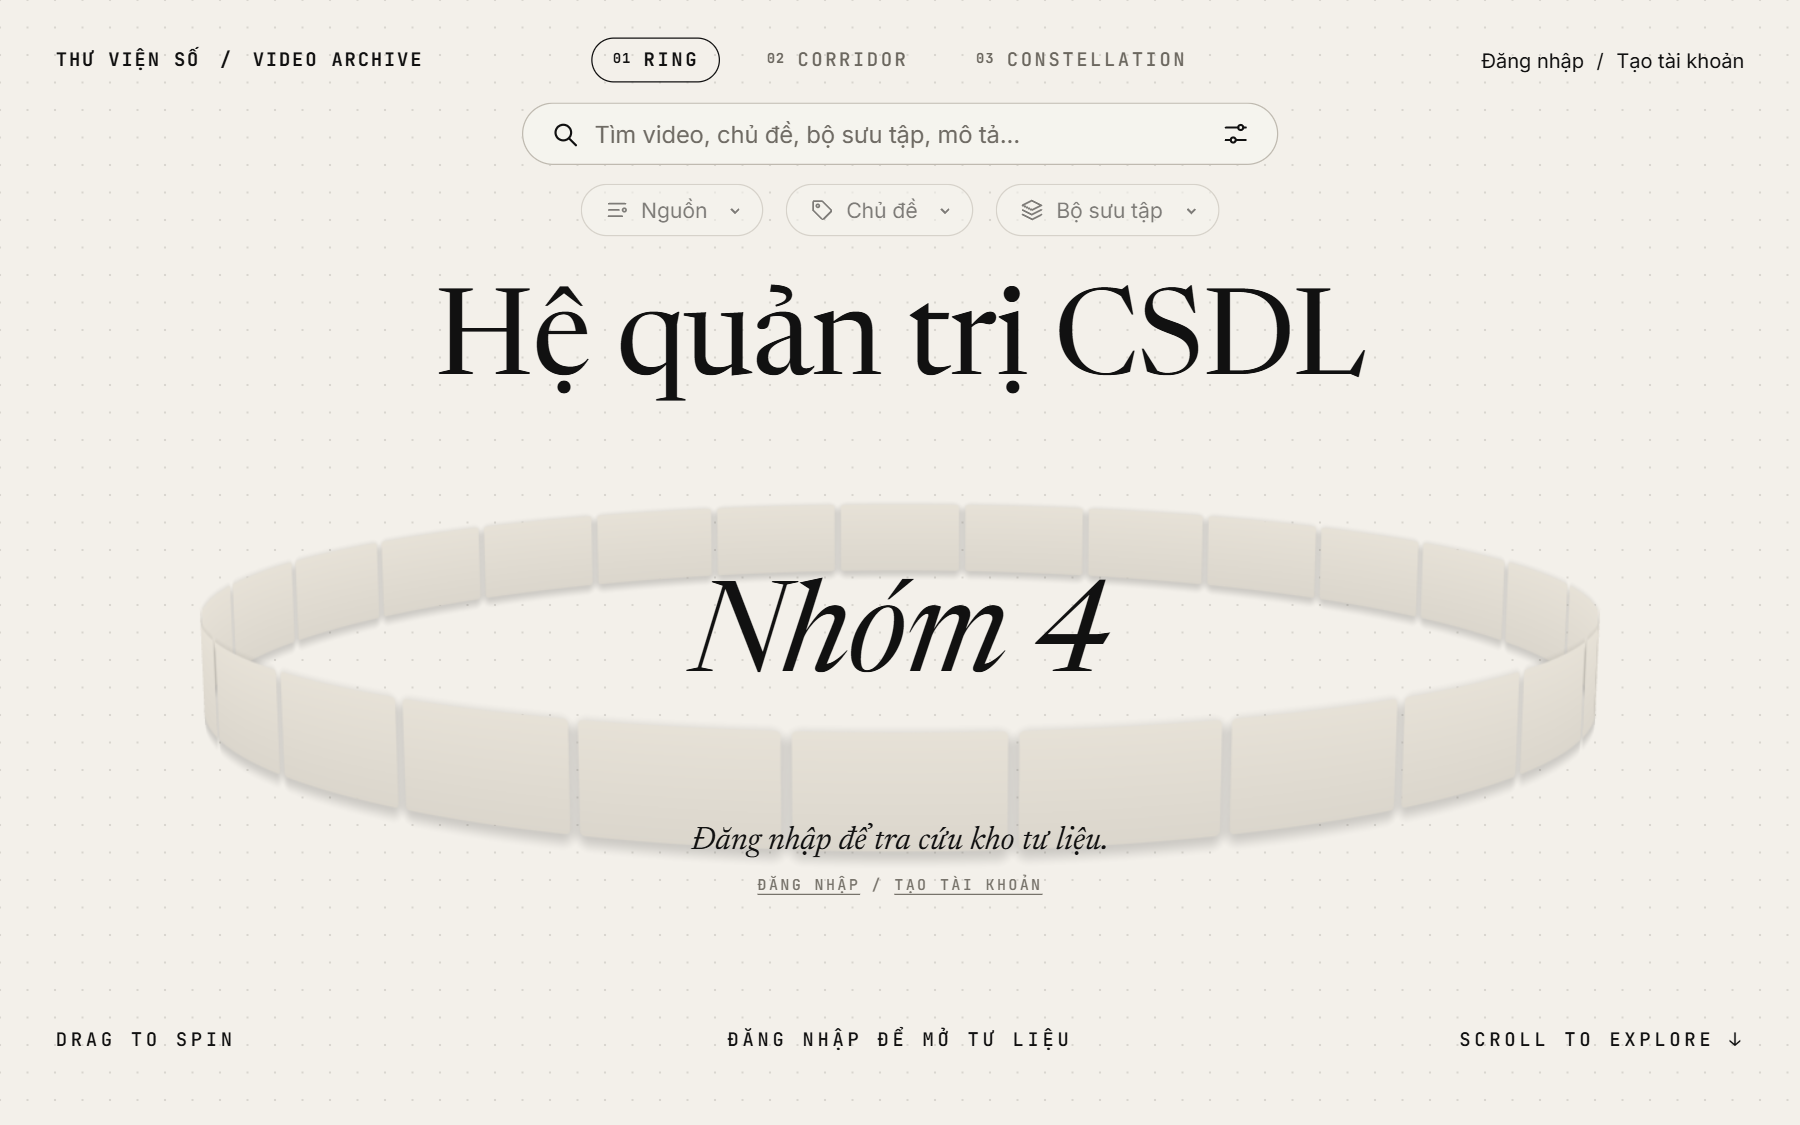
\includegraphics[width=0.9\textwidth]{orbit_landing.png}
\caption{Trang mở đầu công khai: khách chỉ thấy vòng trống, phải đăng nhập mới tra cứu được}
\label{fig:orbit_landing}
\end{figure}

\begin{figure}[H]
\centering
\begin{subfigure}{\textwidth}
\centering
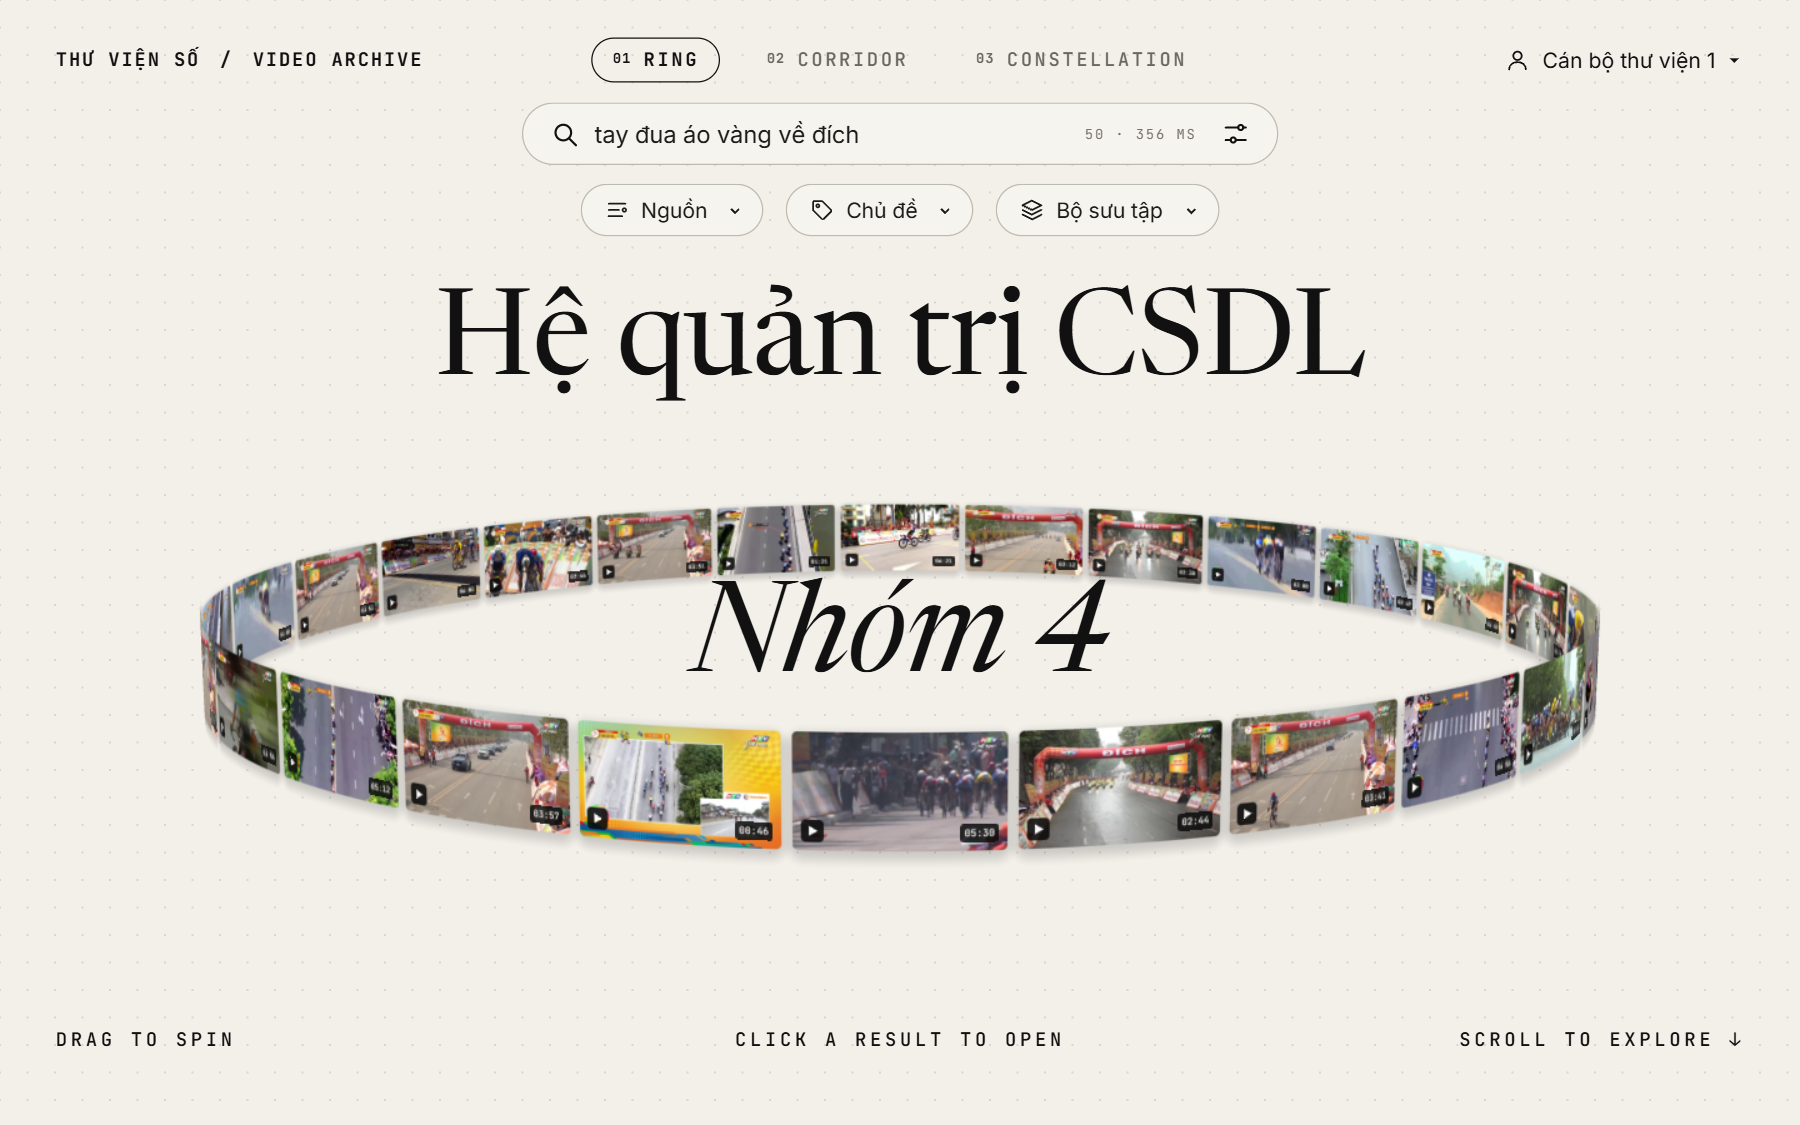
\includegraphics[width=0.82\textwidth]{orbit_ring.png}
\caption{Ring}
\end{subfigure}

\vspace{0.4em}
\begin{subfigure}{0.49\textwidth}
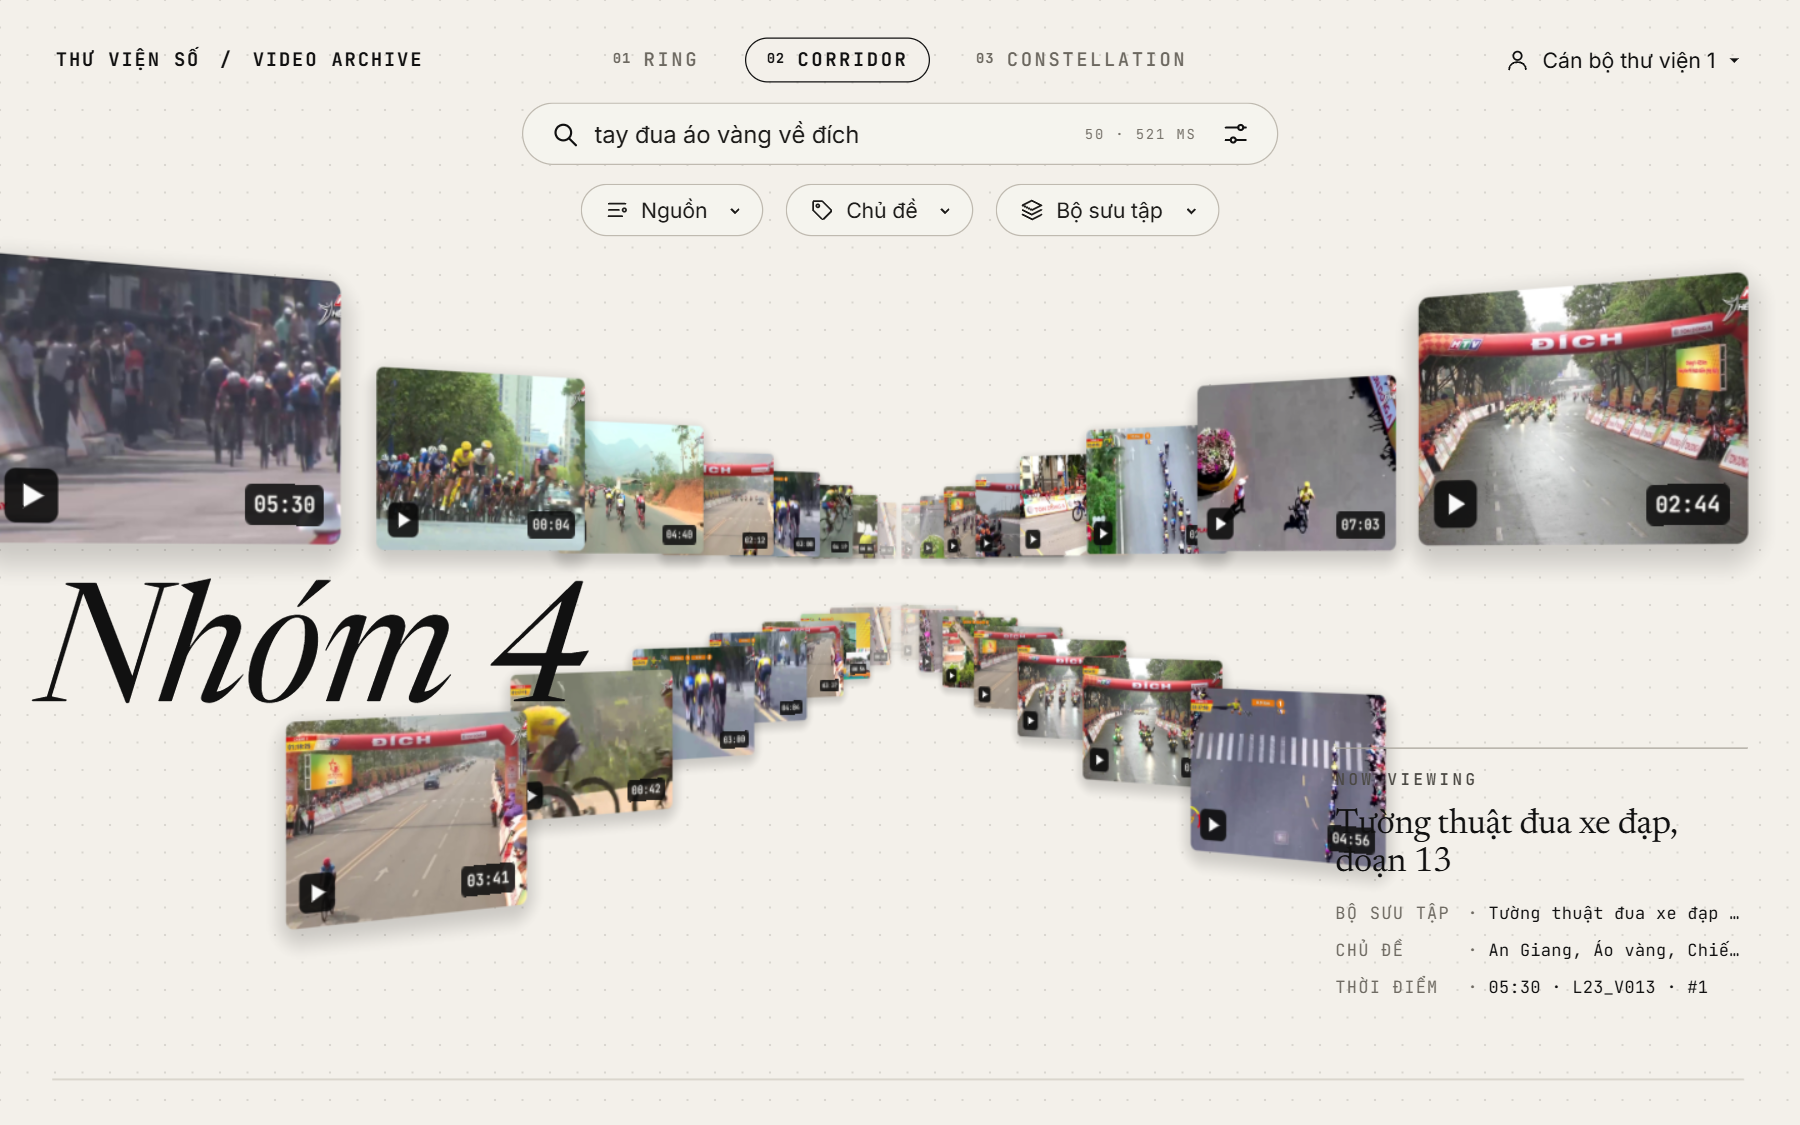
\includegraphics[width=\textwidth]{orbit_corridor.png}
\caption{Corridor}
\end{subfigure}
\hfill
\begin{subfigure}{0.49\textwidth}
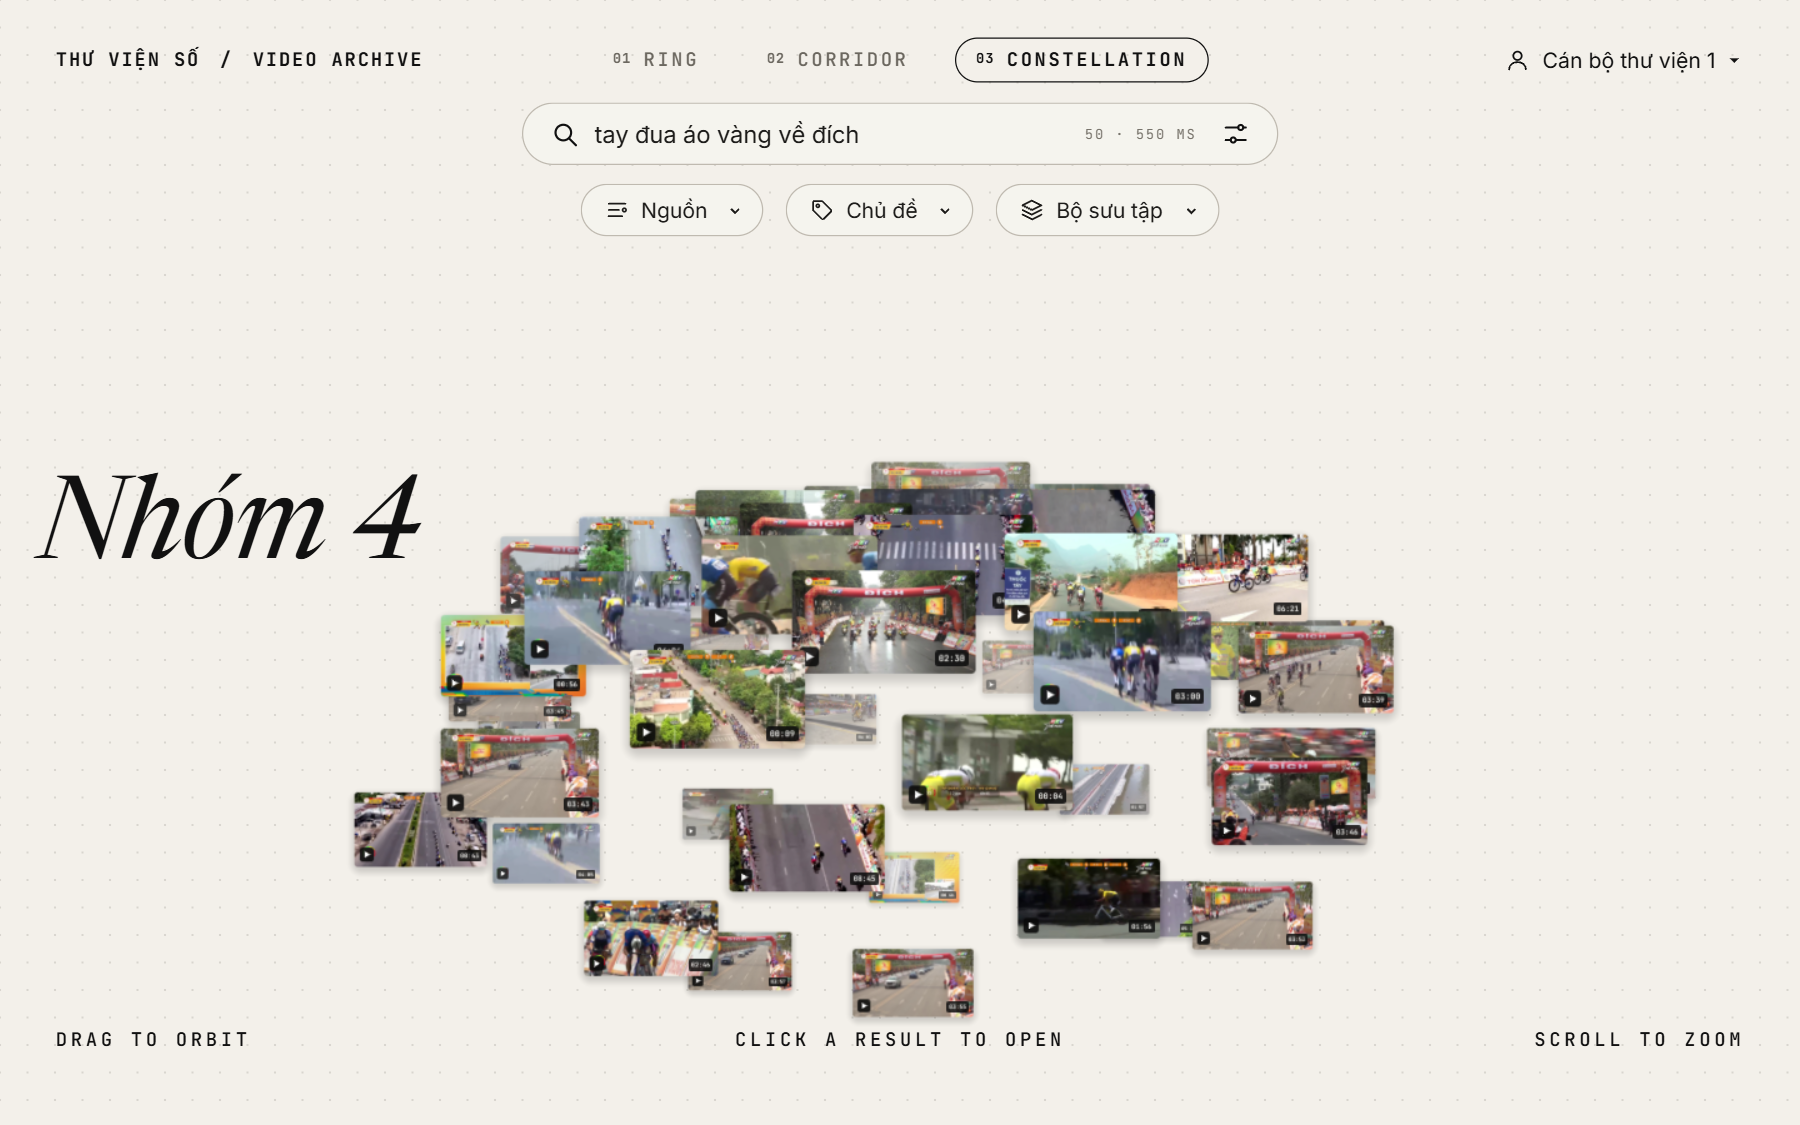
\includegraphics[width=\textwidth]{orbit_constellation.png}
\caption{Constellation}
\end{subfigure}
\caption{Ba chế độ hiển thị cùng một truy vấn ``tay đua áo vàng về đích'' (50 kết quả)}
\label{fig:orbit_views}
\end{figure}

\subsection{Tra cứu dạng danh sách và chi tiết khung hình}

Trang \texttt{/list} giữ dạng lưới truyền thống, thuận tiện khi cần đọc cột bằng chứng của
từng kết quả. Hình~\ref{fig:app_search} là kết quả cán bộ thư viện nhận được cho yêu cầu mẫu
YC-047 (``Người áo trắng chỉ phải cạnh biển HỒNG THÁI PHÚC LỘC''). Khung hình đúng
(L23\_V004, giây 171,8) đứng đầu nhờ chữ OCR (hạng 2 trong nguồn OCR), còn kênh hình ảnh xếp
nó hạng 30. Cả lượt tìm mất 291 ms. Dưới mỗi ảnh là cột \texttt{evidence} do thủ tục trả về.

\begin{figure}[H]
\centering
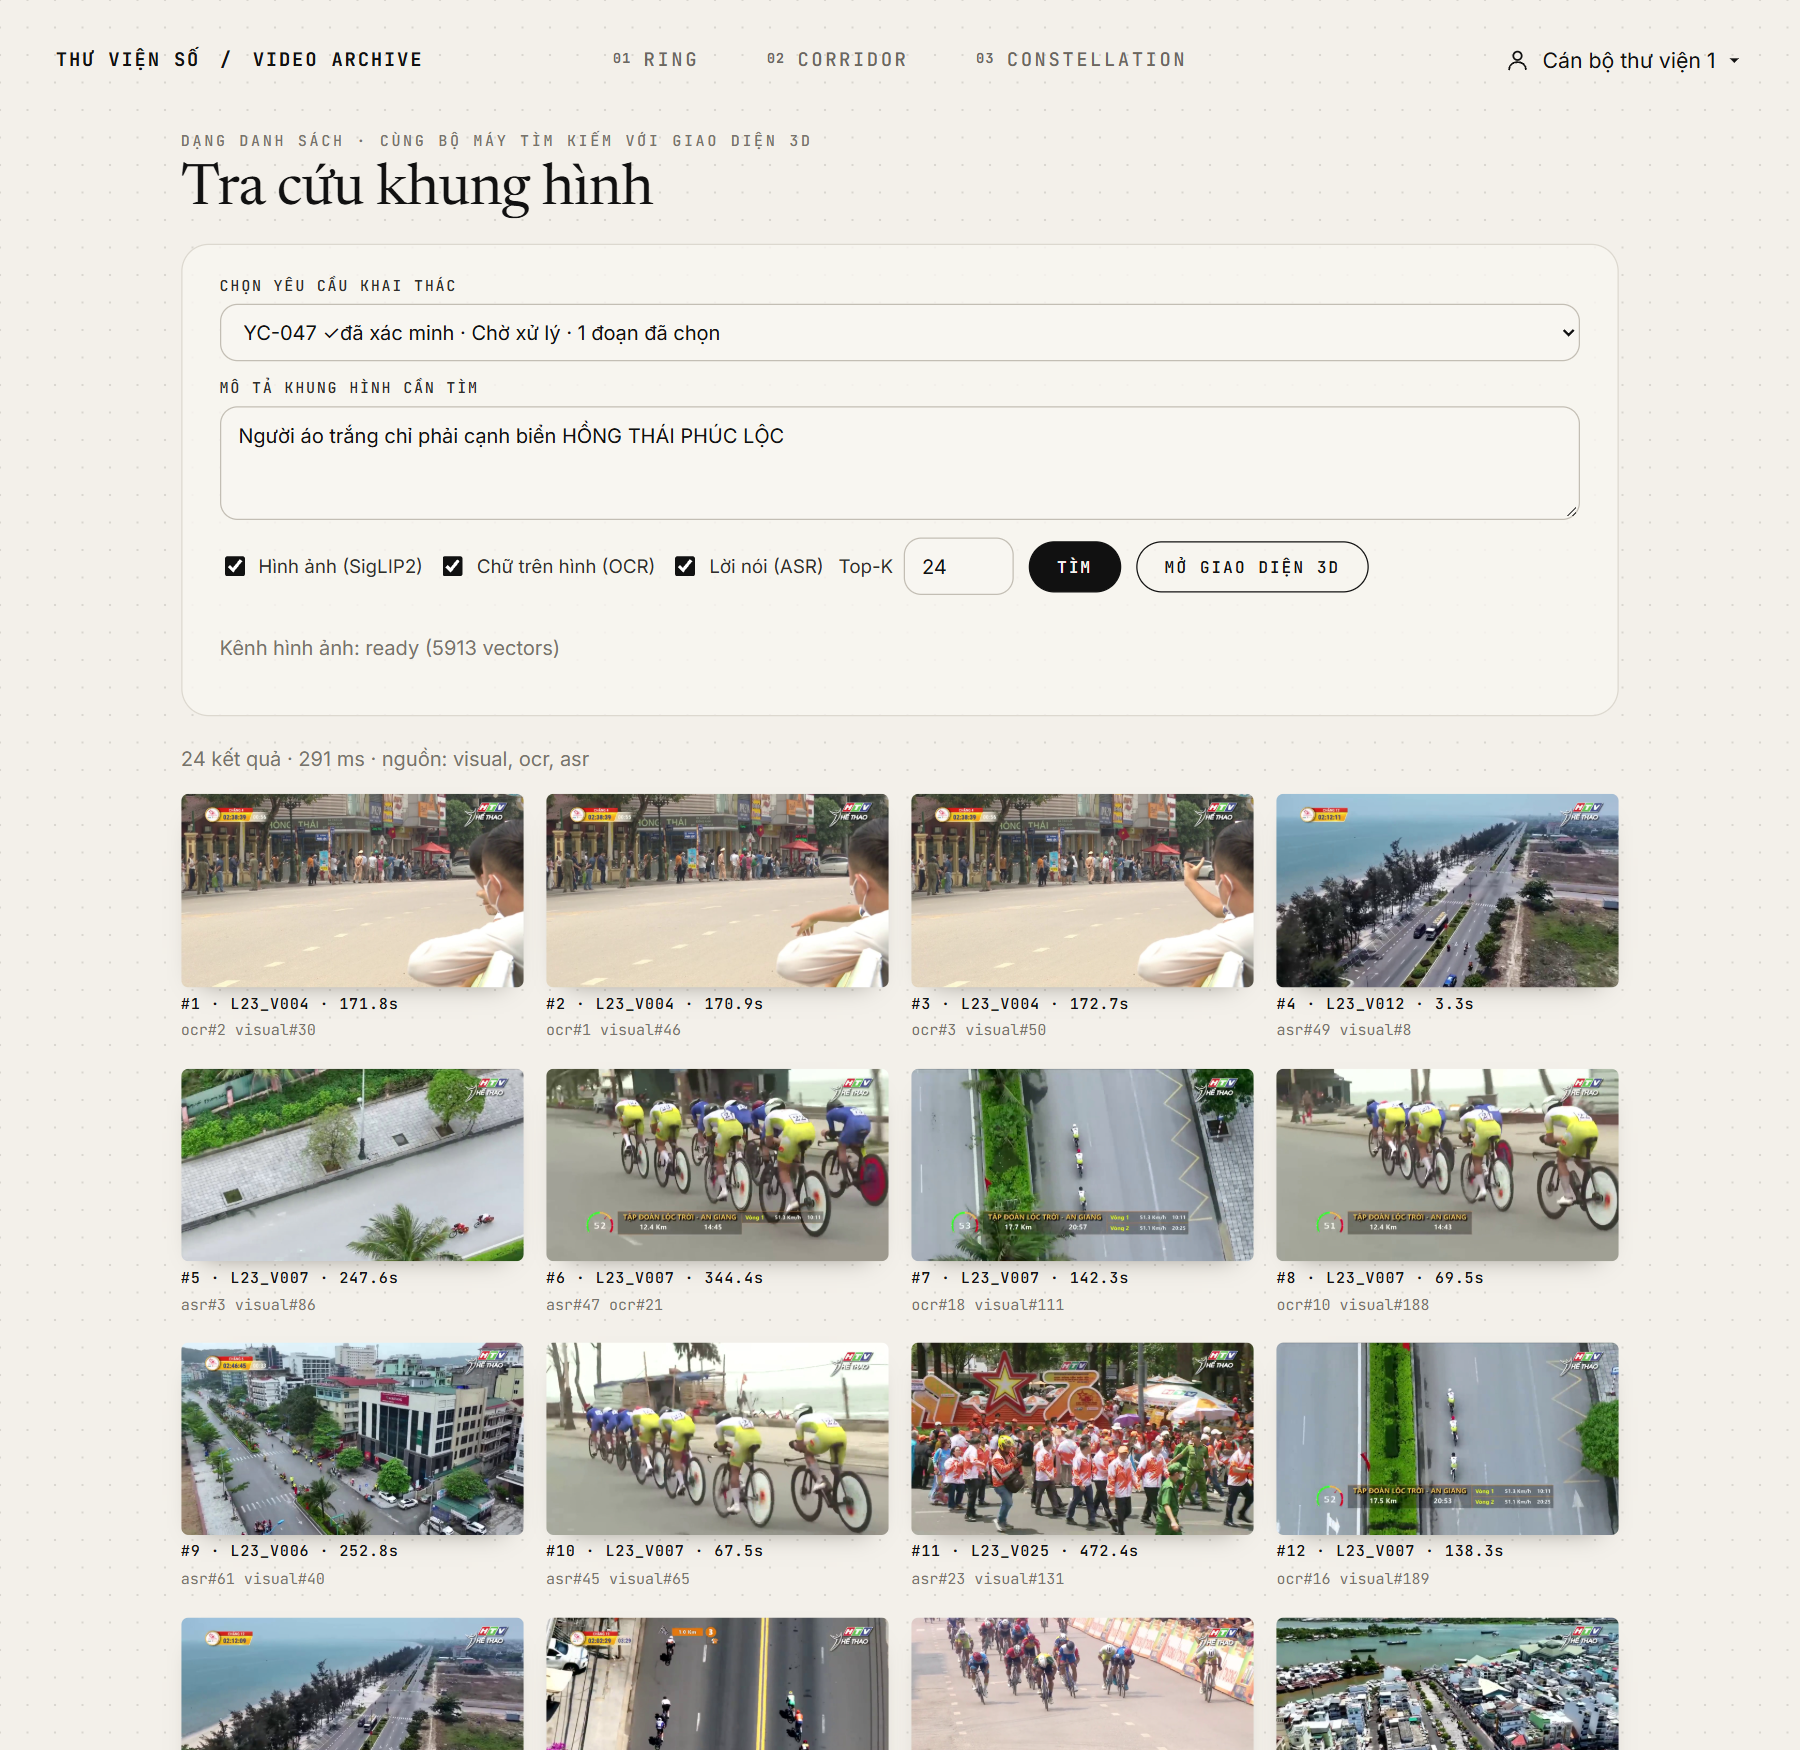
\includegraphics[width=0.9\textwidth]{app_search.png}
\caption{Trang tra cứu dạng danh sách: yêu cầu YC-047 gộp cả ba nguồn, khung hình đúng xếp hạng 1}
\label{fig:app_search}
\end{figure}

\begin{figure}[H]
\centering
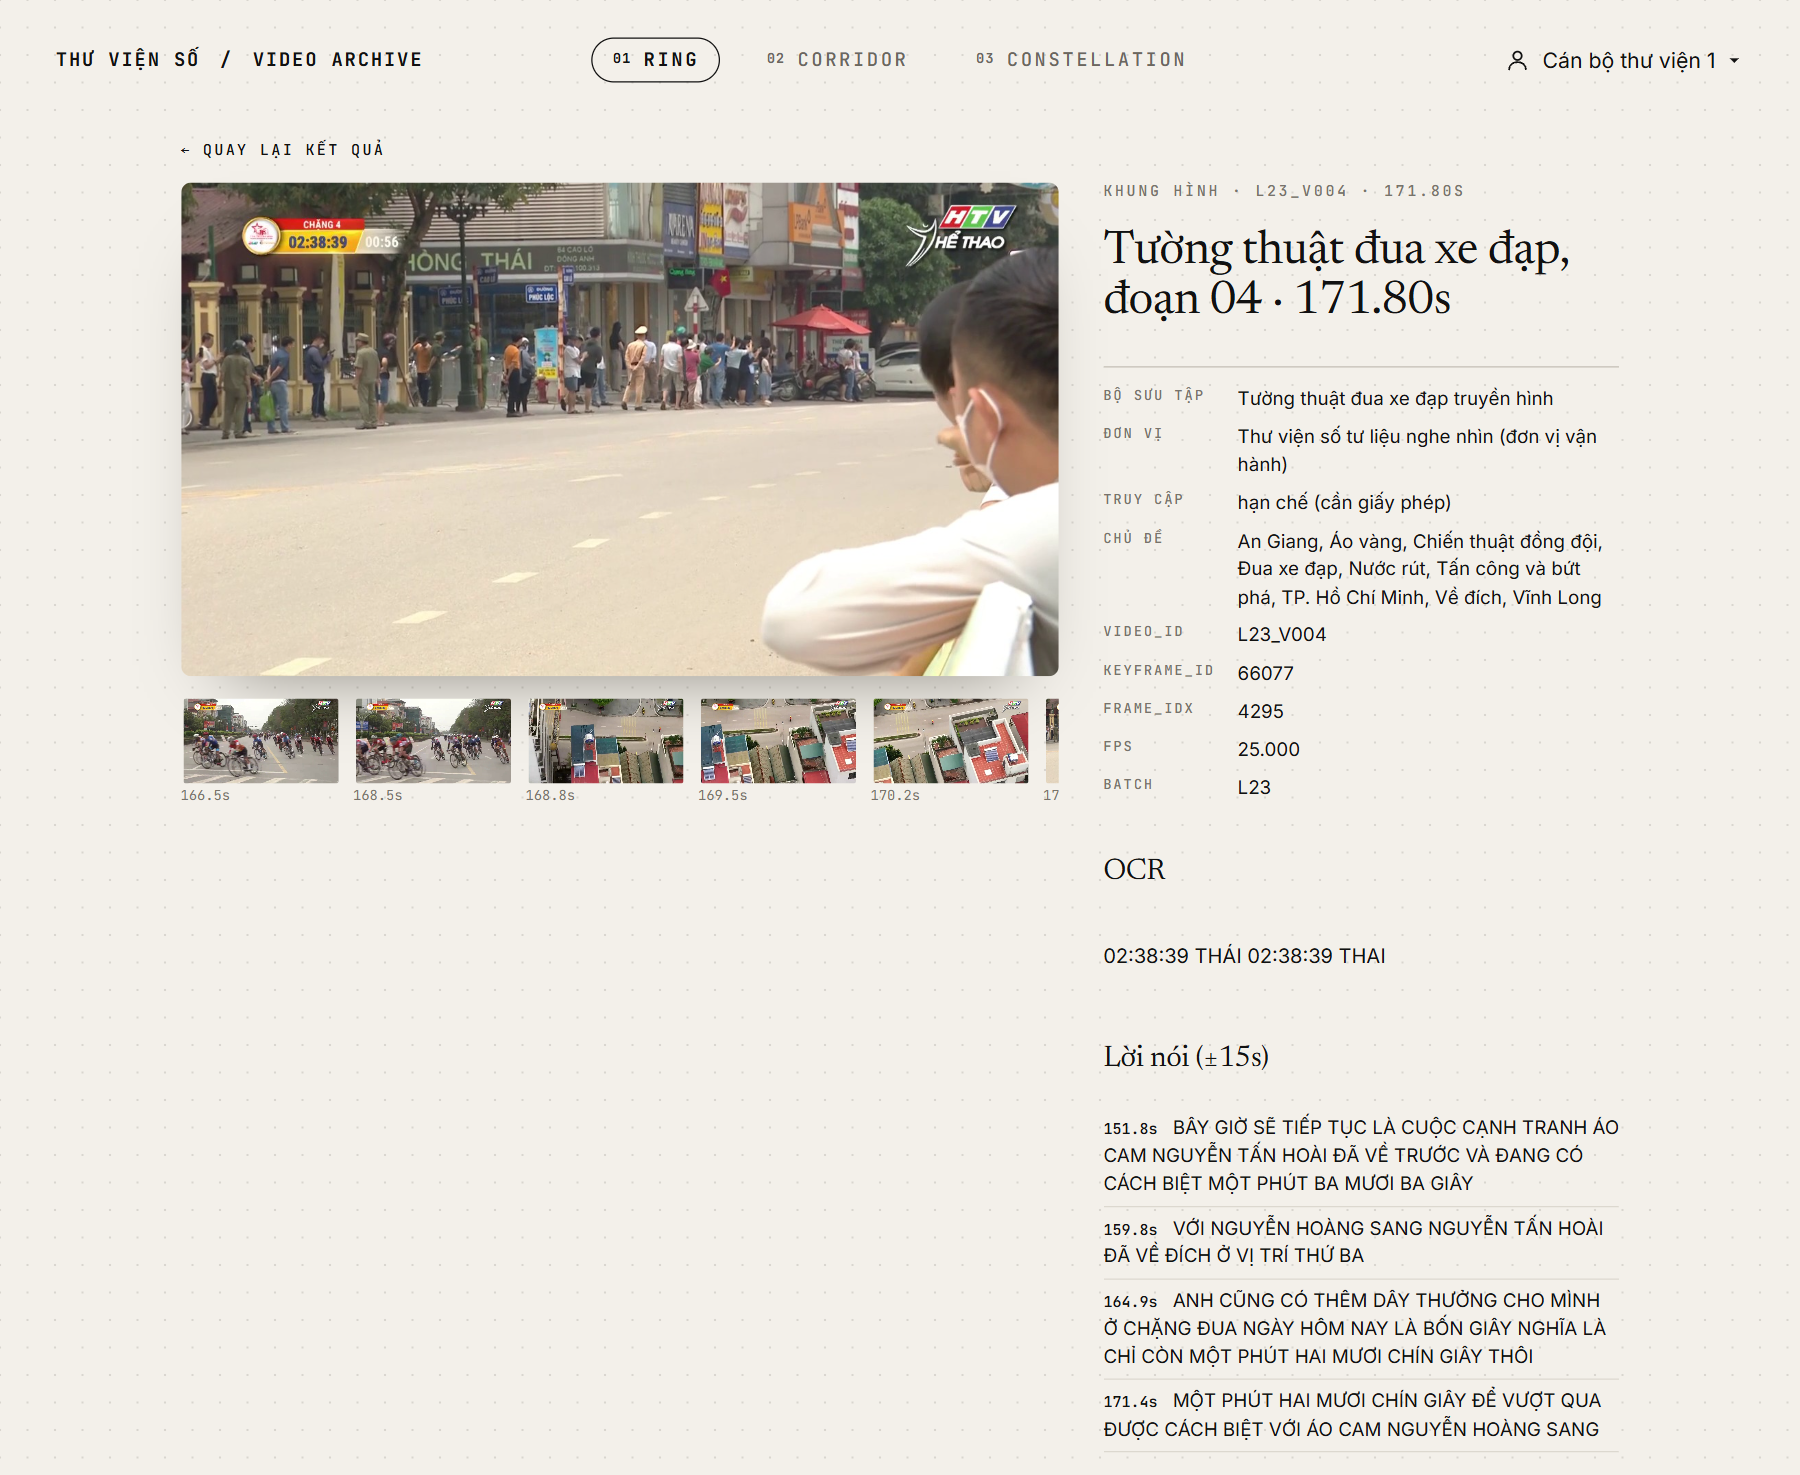
\includegraphics[width=0.9\textwidth]{app_frame.png}
\caption{Trang chi tiết khung hình: phiếu mô tả video (bộ sưu tập, đơn vị, mức truy cập, chủ đề), khung lân cận, chữ OCR, lời nói $\pm$15 giây}
\label{fig:app_frame}
\end{figure}

\subsection{Yêu cầu khai thác}

Trang ``Yêu cầu khai thác'' đọc từ \texttt{v\_request\_progress}. Cán bộ thư viện thấy mọi yêu
cầu, lọc được theo trạng thái, và có nút cấp phép (chọn thời hạn) hoặc từ chối cho yêu cầu
đang chờ; nút cấp phép chỉ hiện khi yêu cầu đã có đoạn tư liệu (Hình~\ref{fig:app_requests}).
Bạn đọc chỉ thấy yêu cầu của mình, có biểu mẫu gửi yêu cầu mới, và tệp CSV xuất ra cũng chỉ
gồm đoạn tư liệu của các yêu cầu đó (Hình~\ref{fig:app_requests_reader}). Nếu ai đó gửi thẳng
yêu cầu HTTP để cấp phép cho một yêu cầu chưa có đoạn nào, thủ tục báo lỗi 50006 và trang
hiển thị thông báo tương ứng.

\begin{figure}[H]
\centering
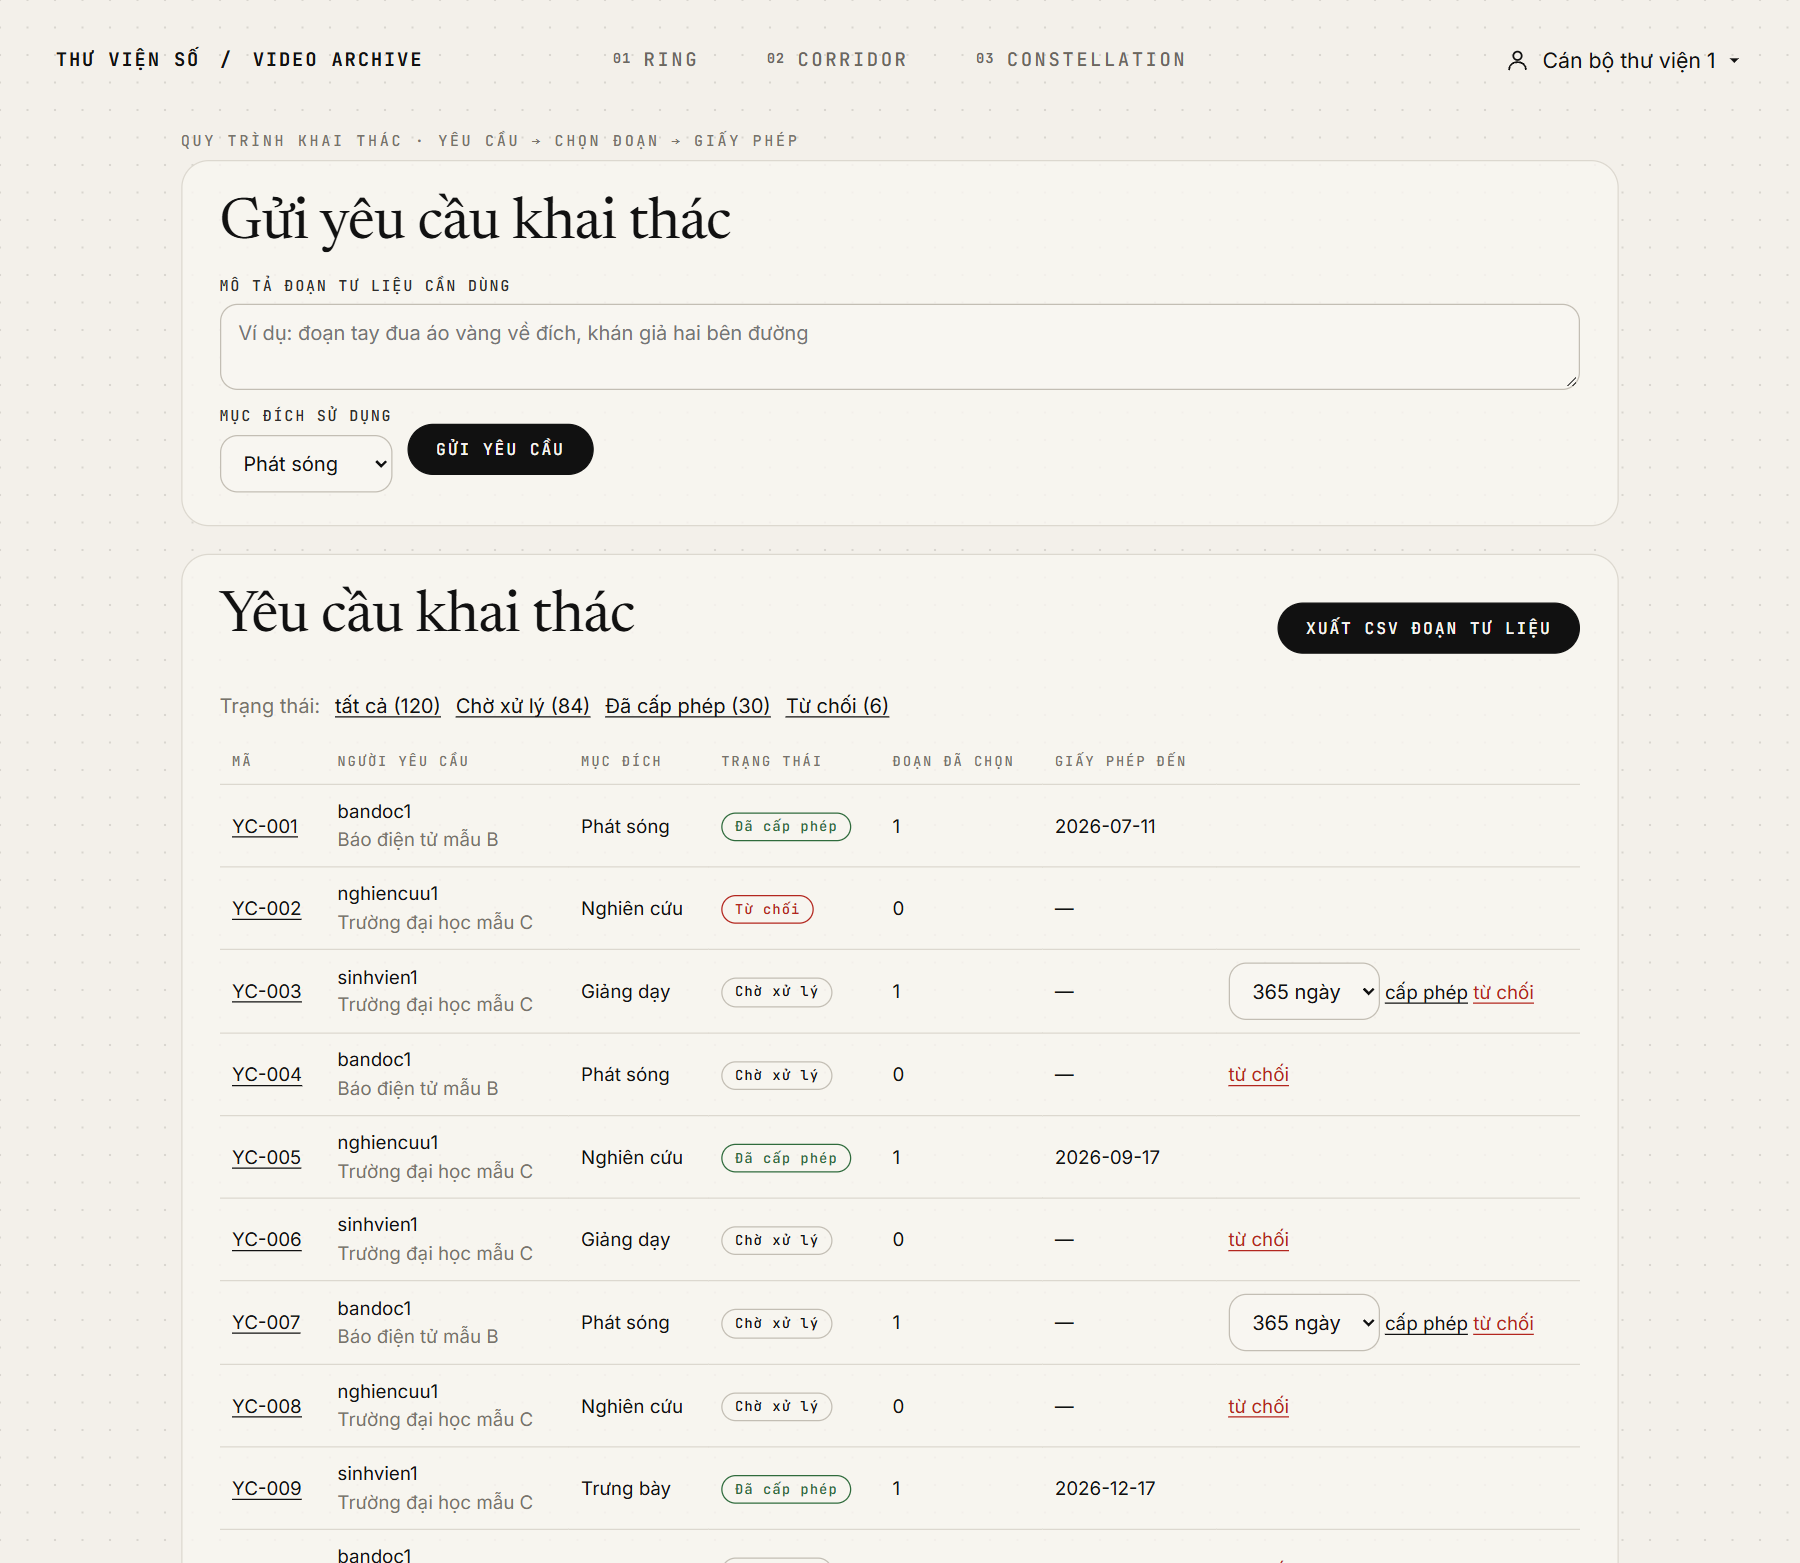
\includegraphics[width=0.9\textwidth]{app_requests.png}
\caption{Trang yêu cầu khai thác của cán bộ thư viện: trạng thái, hạn giấy phép, cấp phép hoặc từ chối}
\label{fig:app_requests}
\end{figure}

\begin{figure}[H]
\centering
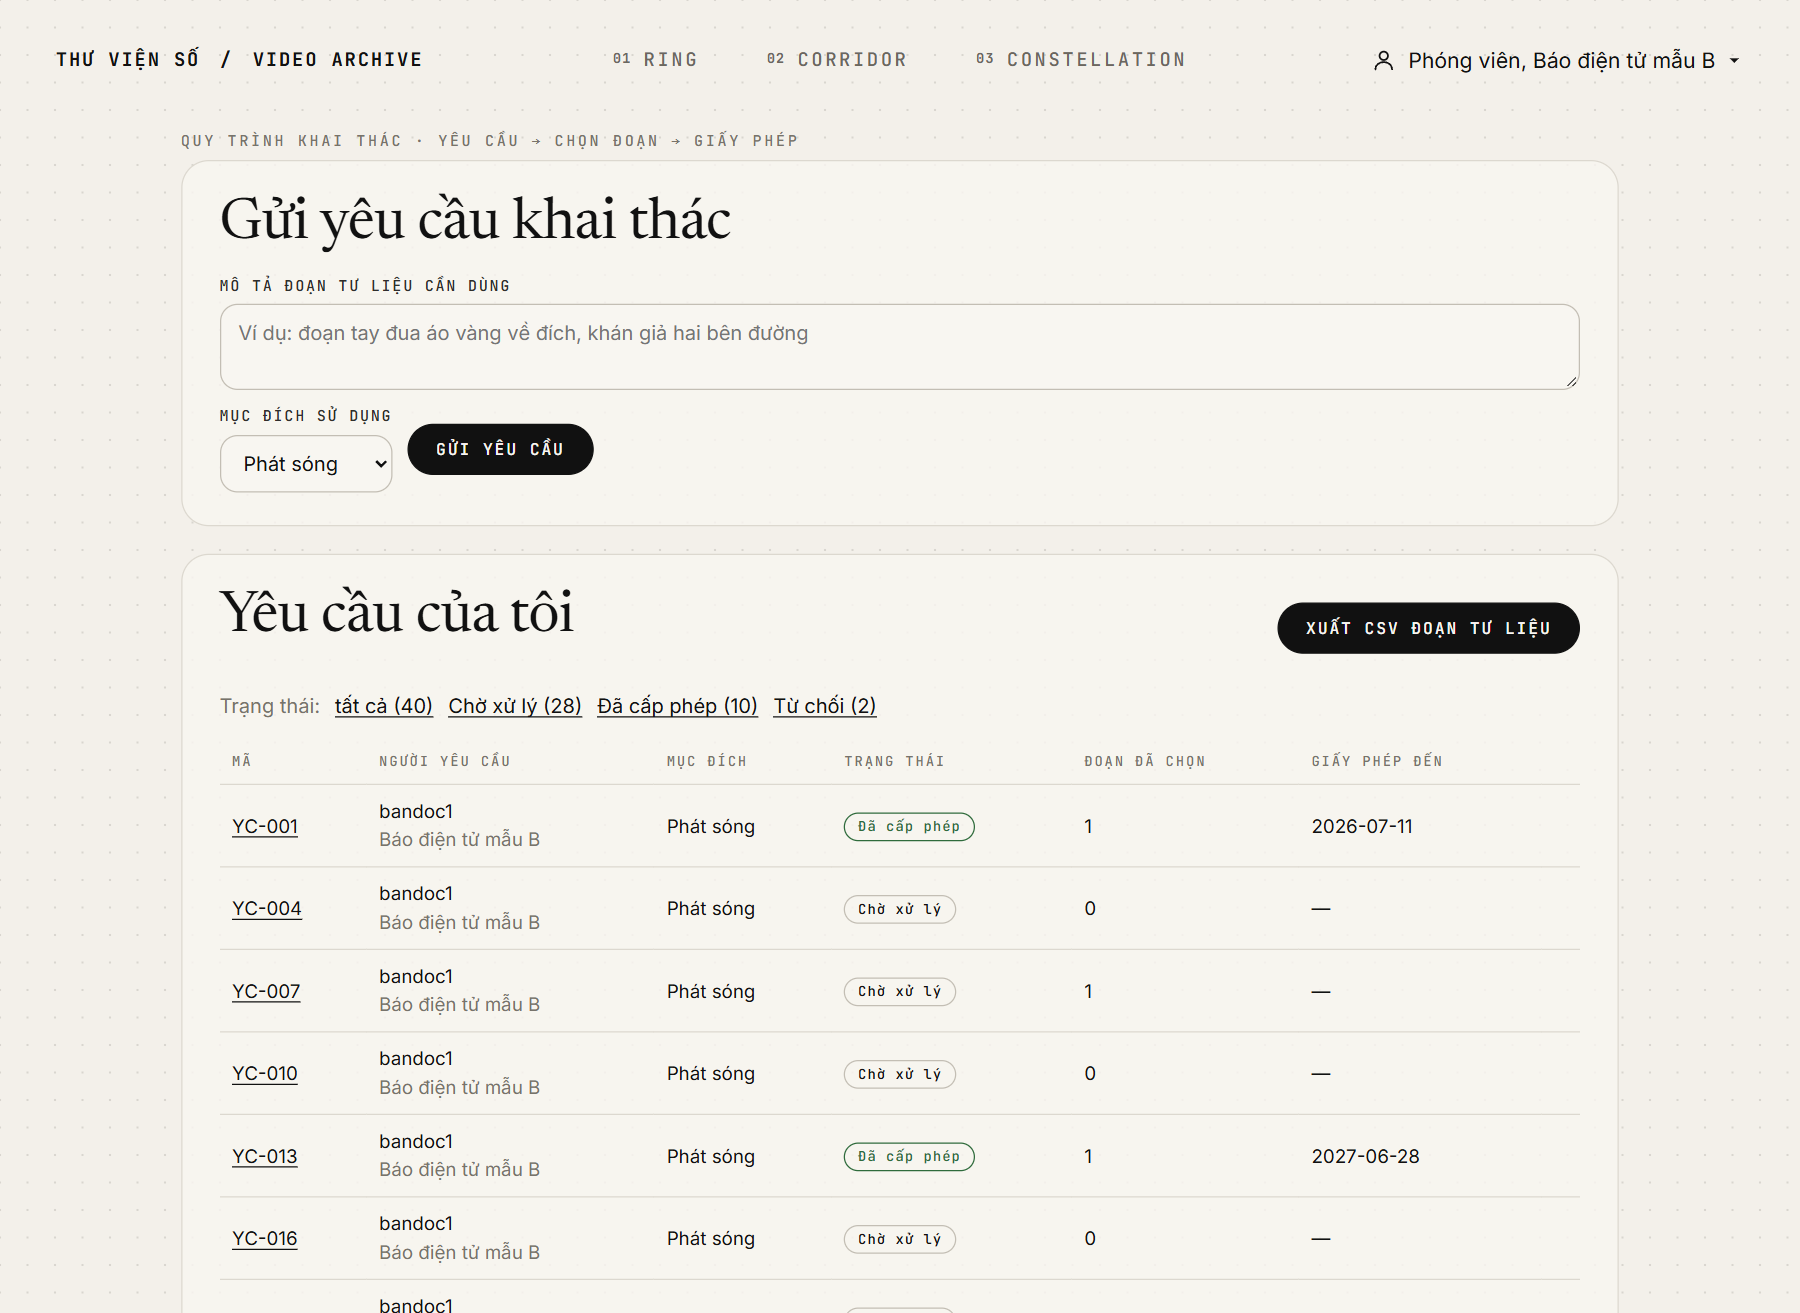
\includegraphics[width=0.9\textwidth]{app_requests_reader.png}
\caption{Cùng trang đó với bạn đọc \texttt{bandoc1}: gửi yêu cầu mới, chỉ thấy 40 yêu cầu của mình}
\label{fig:app_requests_reader}
\end{figure}

\subsection{Tự đăng ký tài khoản bạn đọc}
\label{sec:register}

Khách có thể tự tạo tài khoản bạn đọc ở trang \texttt{/register}
(Hình~\ref{fig:orbit_register}); biến cấu hình \texttt{ARCHIVE\_SELF\_REGISTRATION=0} tắt
trang này và khi đó chỉ quản trị viên tạo được tài khoản. Vì người đăng ký chưa có phiên làm
việc, không thể dựa vào \texttt{SESSION\_CONTEXT} để kiểm tra quyền như các thủ tục ở trên.
Thủ tục \texttt{sp\_register\_reader} vì thế tự khoá cứng những gì được phép:
\begin{itemize}
    \item luôn gán đúng vai trò \texttt{reader}, không nhận tham số vai trò, không gắn đơn vị;
    đối tượng ngoài danh sách (kể cả \texttt{staff}) bị đổi thành \texttt{other};
    \item từ chối mật khẩu chưa băm (giá trị không bắt đầu bằng \texttt{scrypt\$}) với lỗi
    50007, nên dù tầng web có lỗi cũng không lưu được mật khẩu dạng rõ;
    \item thêm người dùng, vai trò và dòng nhật ký \texttt{user.register} trong \textit{một}
    giao dịch.
\end{itemize}
\texttt{archive\_app} chỉ được \texttt{EXECUTE} thủ tục này, không có quyền \texttt{INSERT} trên
\texttt{users}. Ở tầng web, biểu mẫu có mã chống giả mạo yêu cầu (CSRF), mỗi thiết bị tạo tối
đa 5 tài khoản mỗi giờ, và đăng nhập sai 10 lần trong 5 phút thì bị tạm khoá. CSDL đã tạo
trước khi có tính năng này cần chạy thêm \texttt{db/migrations/001\_self\_registration.sql}.

\begin{lstlisting}[caption={Phần lõi của sp\_register\_reader}, label={lst:register}]
IF @user_type IS NULL OR @user_type NOT IN ('journalist', 'researcher', 'student', 'other')
    SET @user_type = 'other';
IF @password_hash IS NULL OR @password_hash NOT LIKE 'scrypt$%'
    THROW 50007, N'Password must be hashed with scrypt', 1;
BEGIN TRY
    BEGIN TRANSACTION;
        INSERT INTO dbo.users (username, full_name, password_hash, organization_id, user_type)
        VALUES (LOWER(LTRIM(RTRIM(@username))), COALESCE(LTRIM(RTRIM(@full_name)), N''),
                @password_hash, NULL, @user_type);
        DECLARE @user_id INT = SCOPE_IDENTITY();
        INSERT INTO dbo.user_roles (user_id, role_id)
        SELECT @user_id, role_id FROM dbo.roles WHERE role_name = 'reader';
        IF @@ROWCOUNT <> 1 THROW 50002, N'Role reader missing', 1;
        INSERT INTO dbo.audit_log (user_id, action, detail)
        VALUES (@user_id, 'user.register', LOWER(LTRIM(RTRIM(@username))));
    COMMIT TRANSACTION;
    SELECT @user_id AS user_id;
END TRY
BEGIN CATCH
    IF @@TRANCOUNT > 0 ROLLBACK TRANSACTION;
    THROW;
END CATCH;
\end{lstlisting}

\begin{figure}[H]
\centering
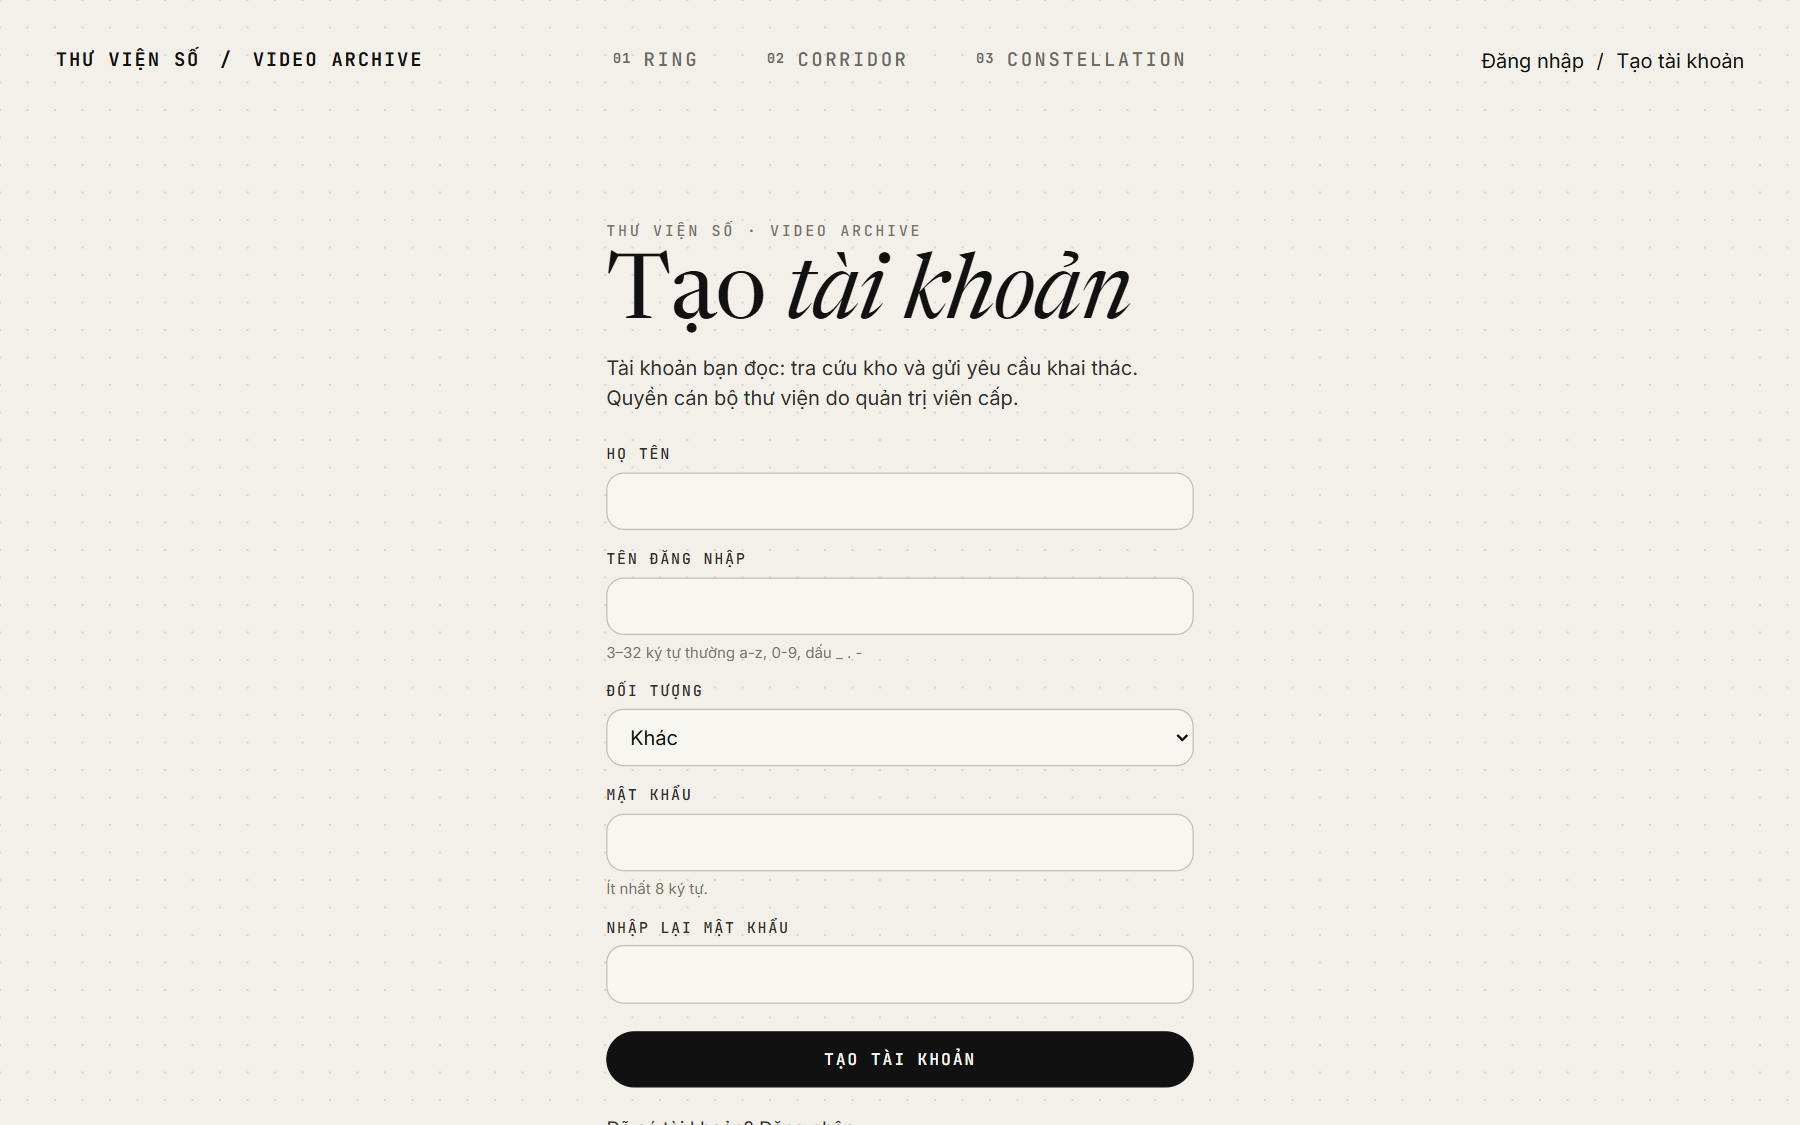
\includegraphics[width=0.75\textwidth]{orbit_register.png}
\caption{Trang tự đăng ký: chỉ tạo được tài khoản bạn đọc}
\label{fig:orbit_register}
\end{figure}

\subsection{Quản trị và đánh giá}

\begin{figure}[H]
\centering
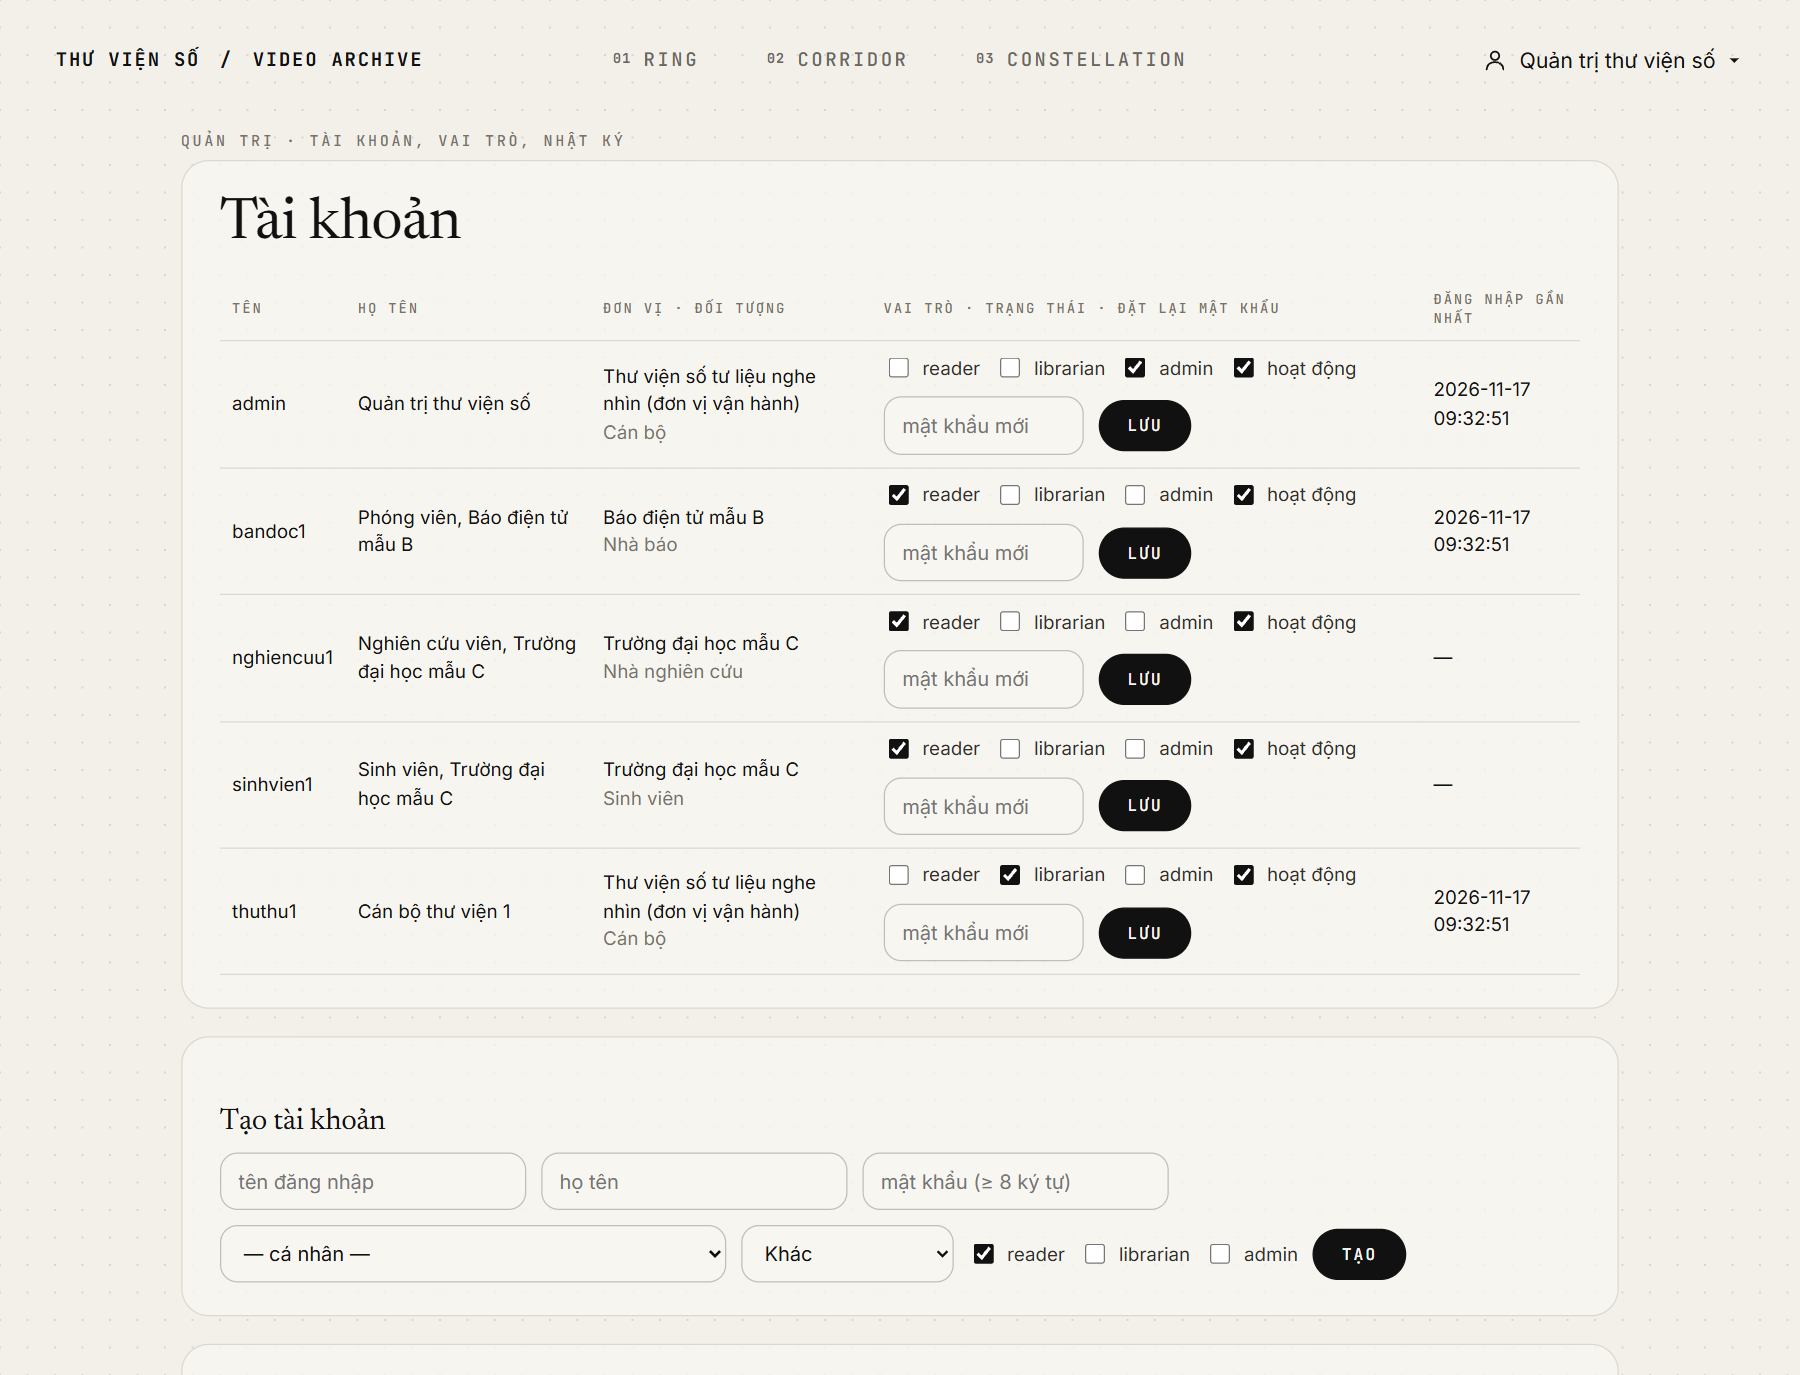
\includegraphics[width=0.9\textwidth]{app_users.png}
\caption{Trang quản trị tài khoản (đơn vị, đối tượng, vai trò) và nhật ký do trigger ghi}
\label{fig:app_users}
\end{figure}

\begin{figure}[H]
\centering
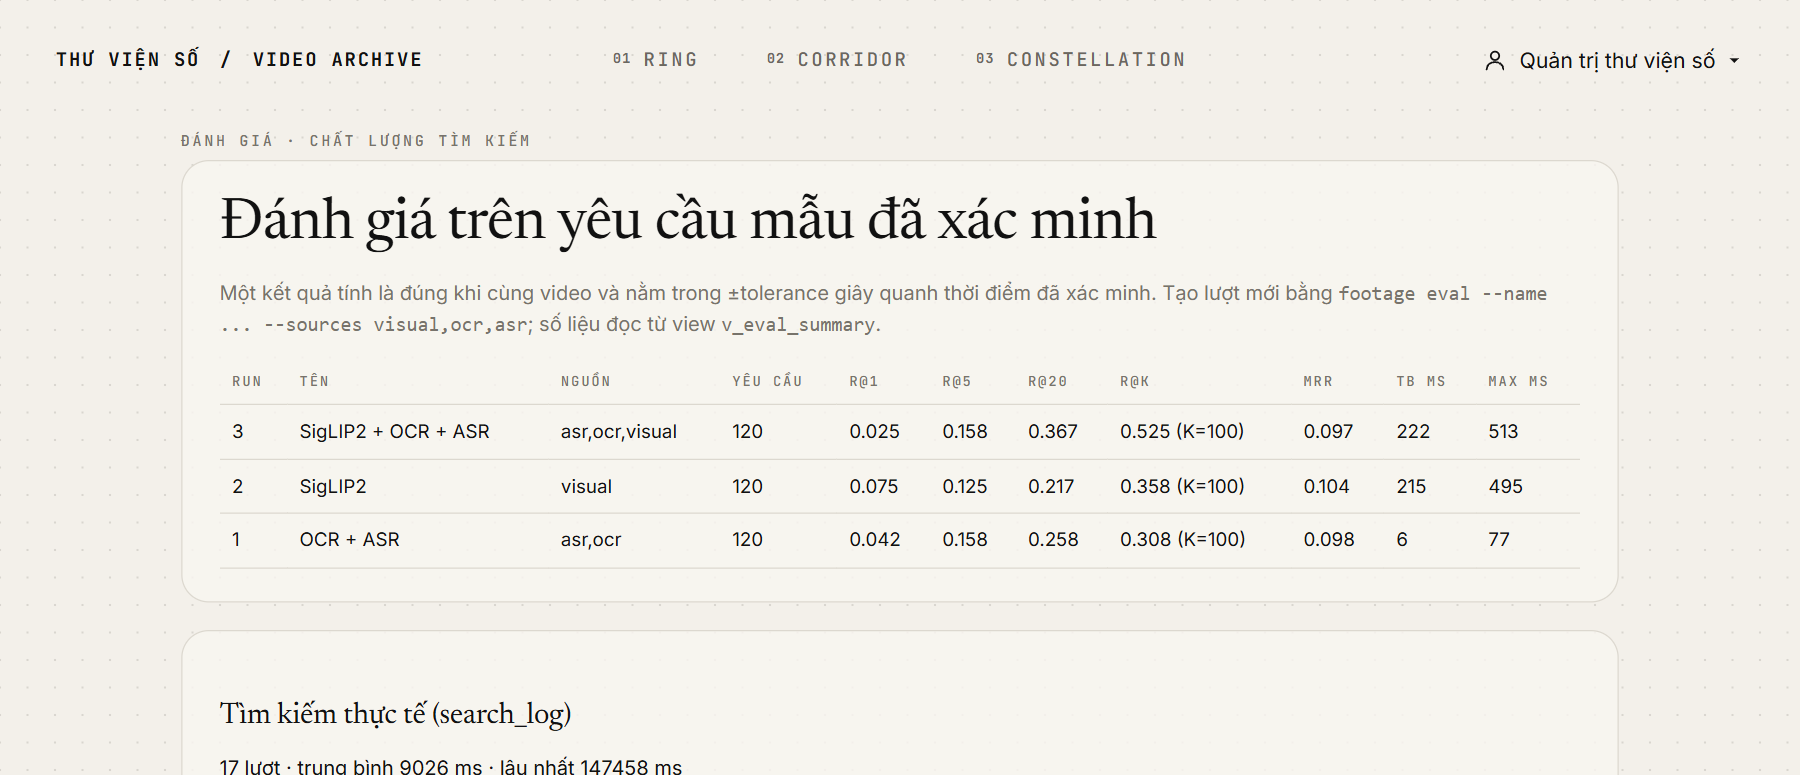
\includegraphics[width=0.9\textwidth]{app_eval.png}
\caption{Trang kết quả đánh giá, đọc từ \texttt{v\_eval\_summary}}
\label{fig:app_misc}
\end{figure}

\section{Đánh giá hiệu quả tìm kiếm}

\subsection{Phương pháp}

Trước khi đưa vào dùng, chất lượng tìm kiếm được đo trên 120 yêu cầu mẫu. Các yêu cầu này
do nhóm tự viết theo cách bạn đọc mô tả đoạn tư liệu cần dùng, và vị trí đúng của từng yêu
cầu được xác minh thủ công. Lệnh \texttt{footage eval} chạy toàn bộ 120 yêu cầu, lưu 100 kết quả
đầu của mỗi yêu cầu vào \texttt{eval\_results}. Một kết quả là đúng nếu cùng video với vị trí
đã xác minh và lệch không quá 3 giây. View \texttt{v\_eval\_summary} tính:
\begin{itemize}
    \item \textbf{Recall@K}: tỉ lệ yêu cầu có ít nhất một kết quả đúng trong $K$ kết quả đầu;
    \item \textbf{MRR}: trung bình của $1/\text{thứ hạng đúng đầu tiên}$ (bằng 0 nếu không tìm thấy);
    \item độ trễ trung bình và lớn nhất của mỗi yêu cầu, tính cả thời gian mã hoá mô tả
    bằng SigLIP2 trên CPU.
\end{itemize}

Kênh hình ảnh dùng chỉ mục SigLIP2 dựng sẵn cho toàn bộ kho: 401.153 vector 1152 chiều, lưu fp16 trong tệp
928 MB. Lệnh \texttt{footage fetch-index} đọc phần đầu tệp bằng HTTP range request để biết vị
trí các mảng dữ liệu, rồi chỉ tải bảng ánh xạ id và đúng 5.913 dòng vector của L23. Tổng
lượng tải khoảng 17 MB thay vì 928 MB. Mọi vector tải về đều có chuẩn bằng 1,000, cho thấy
đã cắt đúng vị trí.

\subsection{Kết quả}

\begin{table}[H]
\centering
\caption{Kết quả trên 120 yêu cầu mẫu đã xác minh (lệch tối đa 3 giây)}
\label{tab:eval}
\renewcommand{\arraystretch}{1.2}
\small
\setlength{\tabcolsep}{5pt}
\begin{tabular}{lrrrrrrr}
\toprule
\textbf{Nguồn} & \textbf{R@1} & \textbf{R@5} & \textbf{R@20} & \textbf{R@100} & \textbf{MRR} & \textbf{TB (ms)} & \textbf{Max (ms)} \\
\midrule
OCR + ASR & 0,042 & 0,158 & 0,258 & 0,308 & 0,098 & 6 & 77 \\
SigLIP2 & 0,075 & 0,125 & 0,217 & 0,358 & 0,104 & 215 & 495 \\
SigLIP2 + OCR + ASR & 0,025 & 0,158 & \textbf{0,367} & \textbf{0,525} & 0,097 & 222 & 513 \\
\bottomrule
\end{tabular}
\end{table}

Nhận xét:
\begin{itemize}
    \item \textbf{Thời gian}: mọi yêu cầu đều xong dưới 0,6 giây, kể cả khi chạy model trên CPU,
    rất xa mốc 30 giây. Riêng phần SQL chỉ mất vài mili giây nhờ chỉ mục ngược.
    \item \textbf{Gộp nguồn}: kết hợp ba nguồn nâng R@100 từ 0,358 (chỉ hình ảnh) lên 0,525
    và R@20 từ 0,217 lên 0,367. Các nguồn bổ sung cho nhau: yêu cầu nhắc tên người hoặc chữ trên
    biển được OCR/ASR tìm thấy, yêu cầu mô tả khung cảnh được hình ảnh tìm thấy.
    \item \textbf{Đánh đổi}: R@1 khi gộp (0,025) thấp hơn khi chỉ dùng hình ảnh (0,075). Với
    trọng số bằng nhau, một khung hình được cả OCR và ASR xếp hạng vừa phải có thể vượt khung
    hình được hình ảnh xếp hạng 1. Có thể khắc phục bằng trọng số riêng cho từng nguồn, nhưng
    cần tập yêu cầu mẫu lớn hơn để tránh tinh chỉnh quá khớp vào 120 yêu cầu này.
    \item \textbf{Thử nghiệm phụ}: viết thường mô tả trước khi mã hoá (theo khuyến nghị
    của SigLIP2) cho kết quả lẫn lộn: R@100 của kênh hình ảnh tăng từ 0,358 lên 0,383 nhưng
    R@1 giảm từ 0,075 xuống 0,050. Vì vậy nhóm giữ nguyên mô tả.
\end{itemize}

\section{Đối chiếu với yêu cầu của đề bài}

\begin{longtable}{>{\raggedright\arraybackslash}p{5.4cm} >{\raggedright\arraybackslash}p{8.6cm}}
\caption{Yêu cầu của đề bài và nơi đáp ứng}\label{tab:requirements}\\
\toprule \textbf{Yêu cầu} & \textbf{Đáp ứng} \\ \midrule \endfirsthead
\toprule \textbf{Yêu cầu} & \textbf{Đáp ứng} \\ \midrule \endhead
\bottomrule \endfoot
Hệ thống ứng dụng tự chọn (không phải quản lý sinh viên) & Thư viện số tư liệu nghe nhìn: danh mục nhiều đơn vị, tra cứu video, yêu cầu khai thác và cấp phép (Chương 1) \\
Script chạy trên SQL Server Express & \texttt{db/full\_setup.sql}, đã chạy trên SQL Server 2025 Express, mức tương thích 140 \\
Tối thiểu 6 bảng chính & 30 bảng, trong đó 22 bảng không phải nhật ký, đánh giá (Bảng~\ref{tab:groups}) \\
Đủ PK, FK, UNIQUE, NOT NULL, DEFAULT, CHECK, đặt tên rõ & 30 PK, 37 FK, 13 UQ, 24 CK, 24 DF, 109 cột NOT NULL (Bảng~\ref{tab:constraint_counts}) \\
30--200 bản ghi để kiểm thử & Dữ liệu thật L23: 5.913 khung hình, 3.976 OCR, 1.238 ASR, 120 yêu cầu khai thác; danh mục minh hoạ: 5 đơn vị, 5 bộ sưu tập, 21 chủ đề, 30 giấy phép \\
Ít nhất 10 truy vấn (JOIN, GROUP BY / HAVING, subquery, UNION / INTERSECT / EXCEPT, LIKE, BETWEEN, TOP / PERCENT) & 25 truy vấn trong \texttt{10\_queries.sql} (Bảng~\ref{tab:queries}), gồm cả INNER, LEFT, RIGHT, FULL JOIN, CTE đệ quy, PIVOT, ROLLUP \\
Tối thiểu 3 stored procedure (có IN/OUT) & 10 thủ tục, \texttt{sp\_progress\_report} có 3 tham số OUTPUT \\
Tối thiểu 2 function & 5 hàm: 3 hàm vô hướng và 2 hàm bảng (một hàm đệ quy), đều được dùng trong truy vấn hoặc thủ tục \\
Tối thiểu 3 view, dùng WITH CHECK OPTION nếu cần & 11 view, \texttt{v\_active\_users} có \texttt{WITH CHECK OPTION} \\
ERD, chuẩn hoá 3NF có nêu các bước & Hình~\ref{fig:erd_catalog}--\ref{fig:erd_logs}, Bảng~\ref{tab:normalization} \\
Kiểm tra vi phạm ràng buộc, giao dịch & \texttt{11\_tests.sql}, mục~\ref{sec:tests}; 67 kiểm thử pytest \\
Chỉ mục cho cột truy vấn thường xuyên & Bảng~\ref{tab:indexes} và~\ref{tab:index_test} \\
README hướng dẫn chạy & \texttt{README.md}, Phụ lục A \\
\end{longtable}
